%\VignetteIndexEntry{PMC Tutorial}
\documentclass{elsarticle}
\usepackage{graphicx, color}
\newcommand{\hlnumber}[1]{\textcolor[rgb]{0,0,0}{#1}}%
\newcommand{\hlfunctioncall}[1]{\textcolor[rgb]{.5,0,.33}{\textbf{#1}}}%
\newcommand{\hlstring}[1]{\textcolor[rgb]{.6,.6,1}{#1}}%
\newcommand{\hlkeyword}[1]{\textbf{#1}}%
\newcommand{\hlargument}[1]{\textcolor[rgb]{.69,.25,.02}{#1}}%
\newcommand{\hlcomment}[1]{\textcolor[rgb]{.18,.6,.34}{#1}}%
\newcommand{\hlroxygencomment}[1]{\textcolor[rgb]{.44,.48,.7}{#1}}%
\newcommand{\hlformalargs}[1]{\hlargument{#1}}%
\newcommand{\hleqformalargs}[1]{\hlargument{#1}}%
\newcommand{\hlassignement}[1]{\textbf{#1}}%
\newcommand{\hlpackage}[1]{\textcolor[rgb]{.59,.71,.145}{#1}}%
\newcommand{\hlslot}[1]{\textit{#1}}%
\newcommand{\hlsymbol}[1]{#1}%
\newcommand{\hlprompt}[1]{\textcolor[rgb]{.5,.5,.5}{#1}}%

\usepackage{color}%
 
\newsavebox{\hlnormalsizeboxclosebrace}%
\newsavebox{\hlnormalsizeboxopenbrace}%
\newsavebox{\hlnormalsizeboxbackslash}%
\newsavebox{\hlnormalsizeboxlessthan}%
\newsavebox{\hlnormalsizeboxgreaterthan}%
\newsavebox{\hlnormalsizeboxdollar}%
\newsavebox{\hlnormalsizeboxunderscore}%
\newsavebox{\hlnormalsizeboxand}%
\newsavebox{\hlnormalsizeboxhash}%
\newsavebox{\hlnormalsizeboxat}%
\newsavebox{\hlnormalsizeboxpercent}% 
\newsavebox{\hlnormalsizeboxhat}%
\newsavebox{\hlnormalsizeboxsinglequote}%
\newsavebox{\hlnormalsizeboxbacktick}%

\setbox\hlnormalsizeboxopenbrace=\hbox{\begin{normalsize}\verb.{.\end{normalsize}}%
\setbox\hlnormalsizeboxclosebrace=\hbox{\begin{normalsize}\verb.}.\end{normalsize}}%
\setbox\hlnormalsizeboxlessthan=\hbox{\begin{normalsize}\verb.<.\end{normalsize}}%
\setbox\hlnormalsizeboxdollar=\hbox{\begin{normalsize}\verb.$.\end{normalsize}}%
\setbox\hlnormalsizeboxunderscore=\hbox{\begin{normalsize}\verb._.\end{normalsize}}%
\setbox\hlnormalsizeboxand=\hbox{\begin{normalsize}\verb.&.\end{normalsize}}%
\setbox\hlnormalsizeboxhash=\hbox{\begin{normalsize}\verb.#.\end{normalsize}}%
\setbox\hlnormalsizeboxat=\hbox{\begin{normalsize}\verb.@.\end{normalsize}}%
\setbox\hlnormalsizeboxbackslash=\hbox{\begin{normalsize}\verb.\.\end{normalsize}}%
\setbox\hlnormalsizeboxgreaterthan=\hbox{\begin{normalsize}\verb.>.\end{normalsize}}%
\setbox\hlnormalsizeboxpercent=\hbox{\begin{normalsize}\verb.%.\end{normalsize}}%
\setbox\hlnormalsizeboxhat=\hbox{\begin{normalsize}\verb.^.\end{normalsize}}%
\setbox\hlnormalsizeboxsinglequote=\hbox{\begin{normalsize}\verb.'.\end{normalsize}}%
\setbox\hlnormalsizeboxbacktick=\hbox{\begin{normalsize}\verb.`.\end{normalsize}}%
\setbox\hlnormalsizeboxhat=\hbox{\begin{normalsize}\verb.^.\end{normalsize}}%



\newsavebox{\hltinyboxclosebrace}%
\newsavebox{\hltinyboxopenbrace}%
\newsavebox{\hltinyboxbackslash}%
\newsavebox{\hltinyboxlessthan}%
\newsavebox{\hltinyboxgreaterthan}%
\newsavebox{\hltinyboxdollar}%
\newsavebox{\hltinyboxunderscore}%
\newsavebox{\hltinyboxand}%
\newsavebox{\hltinyboxhash}%
\newsavebox{\hltinyboxat}%
\newsavebox{\hltinyboxpercent}% 
\newsavebox{\hltinyboxhat}%
\newsavebox{\hltinyboxsinglequote}%
\newsavebox{\hltinyboxbacktick}%

\setbox\hltinyboxopenbrace=\hbox{\begin{tiny}\verb.{.\end{tiny}}%
\setbox\hltinyboxclosebrace=\hbox{\begin{tiny}\verb.}.\end{tiny}}%
\setbox\hltinyboxlessthan=\hbox{\begin{tiny}\verb.<.\end{tiny}}%
\setbox\hltinyboxdollar=\hbox{\begin{tiny}\verb.$.\end{tiny}}%
\setbox\hltinyboxunderscore=\hbox{\begin{tiny}\verb._.\end{tiny}}%
\setbox\hltinyboxand=\hbox{\begin{tiny}\verb.&.\end{tiny}}%
\setbox\hltinyboxhash=\hbox{\begin{tiny}\verb.#.\end{tiny}}%
\setbox\hltinyboxat=\hbox{\begin{tiny}\verb.@.\end{tiny}}%
\setbox\hltinyboxbackslash=\hbox{\begin{tiny}\verb.\.\end{tiny}}%
\setbox\hltinyboxgreaterthan=\hbox{\begin{tiny}\verb.>.\end{tiny}}%
\setbox\hltinyboxpercent=\hbox{\begin{tiny}\verb.%.\end{tiny}}%
\setbox\hltinyboxhat=\hbox{\begin{tiny}\verb.^.\end{tiny}}%
\setbox\hltinyboxsinglequote=\hbox{\begin{tiny}\verb.'.\end{tiny}}%
\setbox\hltinyboxbacktick=\hbox{\begin{tiny}\verb.`.\end{tiny}}%
\setbox\hltinyboxhat=\hbox{\begin{tiny}\verb.^.\end{tiny}}%



\newsavebox{\hlscriptsizeboxclosebrace}%
\newsavebox{\hlscriptsizeboxopenbrace}%
\newsavebox{\hlscriptsizeboxbackslash}%
\newsavebox{\hlscriptsizeboxlessthan}%
\newsavebox{\hlscriptsizeboxgreaterthan}%
\newsavebox{\hlscriptsizeboxdollar}%
\newsavebox{\hlscriptsizeboxunderscore}%
\newsavebox{\hlscriptsizeboxand}%
\newsavebox{\hlscriptsizeboxhash}%
\newsavebox{\hlscriptsizeboxat}%
\newsavebox{\hlscriptsizeboxpercent}% 
\newsavebox{\hlscriptsizeboxhat}%
\newsavebox{\hlscriptsizeboxsinglequote}%
\newsavebox{\hlscriptsizeboxbacktick}%

\setbox\hlscriptsizeboxopenbrace=\hbox{\begin{scriptsize}\verb.{.\end{scriptsize}}%
\setbox\hlscriptsizeboxclosebrace=\hbox{\begin{scriptsize}\verb.}.\end{scriptsize}}%
\setbox\hlscriptsizeboxlessthan=\hbox{\begin{scriptsize}\verb.<.\end{scriptsize}}%
\setbox\hlscriptsizeboxdollar=\hbox{\begin{scriptsize}\verb.$.\end{scriptsize}}%
\setbox\hlscriptsizeboxunderscore=\hbox{\begin{scriptsize}\verb._.\end{scriptsize}}%
\setbox\hlscriptsizeboxand=\hbox{\begin{scriptsize}\verb.&.\end{scriptsize}}%
\setbox\hlscriptsizeboxhash=\hbox{\begin{scriptsize}\verb.#.\end{scriptsize}}%
\setbox\hlscriptsizeboxat=\hbox{\begin{scriptsize}\verb.@.\end{scriptsize}}%
\setbox\hlscriptsizeboxbackslash=\hbox{\begin{scriptsize}\verb.\.\end{scriptsize}}%
\setbox\hlscriptsizeboxgreaterthan=\hbox{\begin{scriptsize}\verb.>.\end{scriptsize}}%
\setbox\hlscriptsizeboxpercent=\hbox{\begin{scriptsize}\verb.%.\end{scriptsize}}%
\setbox\hlscriptsizeboxhat=\hbox{\begin{scriptsize}\verb.^.\end{scriptsize}}%
\setbox\hlscriptsizeboxsinglequote=\hbox{\begin{scriptsize}\verb.'.\end{scriptsize}}%
\setbox\hlscriptsizeboxbacktick=\hbox{\begin{scriptsize}\verb.`.\end{scriptsize}}%
\setbox\hlscriptsizeboxhat=\hbox{\begin{scriptsize}\verb.^.\end{scriptsize}}%



\newsavebox{\hlfootnotesizeboxclosebrace}%
\newsavebox{\hlfootnotesizeboxopenbrace}%
\newsavebox{\hlfootnotesizeboxbackslash}%
\newsavebox{\hlfootnotesizeboxlessthan}%
\newsavebox{\hlfootnotesizeboxgreaterthan}%
\newsavebox{\hlfootnotesizeboxdollar}%
\newsavebox{\hlfootnotesizeboxunderscore}%
\newsavebox{\hlfootnotesizeboxand}%
\newsavebox{\hlfootnotesizeboxhash}%
\newsavebox{\hlfootnotesizeboxat}%
\newsavebox{\hlfootnotesizeboxpercent}% 
\newsavebox{\hlfootnotesizeboxhat}%
\newsavebox{\hlfootnotesizeboxsinglequote}%
\newsavebox{\hlfootnotesizeboxbacktick}%

\setbox\hlfootnotesizeboxopenbrace=\hbox{\begin{footnotesize}\verb.{.\end{footnotesize}}%
\setbox\hlfootnotesizeboxclosebrace=\hbox{\begin{footnotesize}\verb.}.\end{footnotesize}}%
\setbox\hlfootnotesizeboxlessthan=\hbox{\begin{footnotesize}\verb.<.\end{footnotesize}}%
\setbox\hlfootnotesizeboxdollar=\hbox{\begin{footnotesize}\verb.$.\end{footnotesize}}%
\setbox\hlfootnotesizeboxunderscore=\hbox{\begin{footnotesize}\verb._.\end{footnotesize}}%
\setbox\hlfootnotesizeboxand=\hbox{\begin{footnotesize}\verb.&.\end{footnotesize}}%
\setbox\hlfootnotesizeboxhash=\hbox{\begin{footnotesize}\verb.#.\end{footnotesize}}%
\setbox\hlfootnotesizeboxat=\hbox{\begin{footnotesize}\verb.@.\end{footnotesize}}%
\setbox\hlfootnotesizeboxbackslash=\hbox{\begin{footnotesize}\verb.\.\end{footnotesize}}%
\setbox\hlfootnotesizeboxgreaterthan=\hbox{\begin{footnotesize}\verb.>.\end{footnotesize}}%
\setbox\hlfootnotesizeboxpercent=\hbox{\begin{footnotesize}\verb.%.\end{footnotesize}}%
\setbox\hlfootnotesizeboxhat=\hbox{\begin{footnotesize}\verb.^.\end{footnotesize}}%
\setbox\hlfootnotesizeboxsinglequote=\hbox{\begin{footnotesize}\verb.'.\end{footnotesize}}%
\setbox\hlfootnotesizeboxbacktick=\hbox{\begin{footnotesize}\verb.`.\end{footnotesize}}%
\setbox\hlfootnotesizeboxhat=\hbox{\begin{footnotesize}\verb.^.\end{footnotesize}}%



\newsavebox{\hlsmallboxclosebrace}%
\newsavebox{\hlsmallboxopenbrace}%
\newsavebox{\hlsmallboxbackslash}%
\newsavebox{\hlsmallboxlessthan}%
\newsavebox{\hlsmallboxgreaterthan}%
\newsavebox{\hlsmallboxdollar}%
\newsavebox{\hlsmallboxunderscore}%
\newsavebox{\hlsmallboxand}%
\newsavebox{\hlsmallboxhash}%
\newsavebox{\hlsmallboxat}%
\newsavebox{\hlsmallboxpercent}% 
\newsavebox{\hlsmallboxhat}%
\newsavebox{\hlsmallboxsinglequote}%
\newsavebox{\hlsmallboxbacktick}%

\setbox\hlsmallboxopenbrace=\hbox{\begin{small}\verb.{.\end{small}}%
\setbox\hlsmallboxclosebrace=\hbox{\begin{small}\verb.}.\end{small}}%
\setbox\hlsmallboxlessthan=\hbox{\begin{small}\verb.<.\end{small}}%
\setbox\hlsmallboxdollar=\hbox{\begin{small}\verb.$.\end{small}}%
\setbox\hlsmallboxunderscore=\hbox{\begin{small}\verb._.\end{small}}%
\setbox\hlsmallboxand=\hbox{\begin{small}\verb.&.\end{small}}%
\setbox\hlsmallboxhash=\hbox{\begin{small}\verb.#.\end{small}}%
\setbox\hlsmallboxat=\hbox{\begin{small}\verb.@.\end{small}}%
\setbox\hlsmallboxbackslash=\hbox{\begin{small}\verb.\.\end{small}}%
\setbox\hlsmallboxgreaterthan=\hbox{\begin{small}\verb.>.\end{small}}%
\setbox\hlsmallboxpercent=\hbox{\begin{small}\verb.%.\end{small}}%
\setbox\hlsmallboxhat=\hbox{\begin{small}\verb.^.\end{small}}%
\setbox\hlsmallboxsinglequote=\hbox{\begin{small}\verb.'.\end{small}}%
\setbox\hlsmallboxbacktick=\hbox{\begin{small}\verb.`.\end{small}}%
\setbox\hlsmallboxhat=\hbox{\begin{small}\verb.^.\end{small}}%



\newsavebox{\hllargeboxclosebrace}%
\newsavebox{\hllargeboxopenbrace}%
\newsavebox{\hllargeboxbackslash}%
\newsavebox{\hllargeboxlessthan}%
\newsavebox{\hllargeboxgreaterthan}%
\newsavebox{\hllargeboxdollar}%
\newsavebox{\hllargeboxunderscore}%
\newsavebox{\hllargeboxand}%
\newsavebox{\hllargeboxhash}%
\newsavebox{\hllargeboxat}%
\newsavebox{\hllargeboxpercent}% 
\newsavebox{\hllargeboxhat}%
\newsavebox{\hllargeboxsinglequote}%
\newsavebox{\hllargeboxbacktick}%

\setbox\hllargeboxopenbrace=\hbox{\begin{large}\verb.{.\end{large}}%
\setbox\hllargeboxclosebrace=\hbox{\begin{large}\verb.}.\end{large}}%
\setbox\hllargeboxlessthan=\hbox{\begin{large}\verb.<.\end{large}}%
\setbox\hllargeboxdollar=\hbox{\begin{large}\verb.$.\end{large}}%
\setbox\hllargeboxunderscore=\hbox{\begin{large}\verb._.\end{large}}%
\setbox\hllargeboxand=\hbox{\begin{large}\verb.&.\end{large}}%
\setbox\hllargeboxhash=\hbox{\begin{large}\verb.#.\end{large}}%
\setbox\hllargeboxat=\hbox{\begin{large}\verb.@.\end{large}}%
\setbox\hllargeboxbackslash=\hbox{\begin{large}\verb.\.\end{large}}%
\setbox\hllargeboxgreaterthan=\hbox{\begin{large}\verb.>.\end{large}}%
\setbox\hllargeboxpercent=\hbox{\begin{large}\verb.%.\end{large}}%
\setbox\hllargeboxhat=\hbox{\begin{large}\verb.^.\end{large}}%
\setbox\hllargeboxsinglequote=\hbox{\begin{large}\verb.'.\end{large}}%
\setbox\hllargeboxbacktick=\hbox{\begin{large}\verb.`.\end{large}}%
\setbox\hllargeboxhat=\hbox{\begin{large}\verb.^.\end{large}}%



\newsavebox{\hlLargeboxclosebrace}%
\newsavebox{\hlLargeboxopenbrace}%
\newsavebox{\hlLargeboxbackslash}%
\newsavebox{\hlLargeboxlessthan}%
\newsavebox{\hlLargeboxgreaterthan}%
\newsavebox{\hlLargeboxdollar}%
\newsavebox{\hlLargeboxunderscore}%
\newsavebox{\hlLargeboxand}%
\newsavebox{\hlLargeboxhash}%
\newsavebox{\hlLargeboxat}%
\newsavebox{\hlLargeboxpercent}% 
\newsavebox{\hlLargeboxhat}%
\newsavebox{\hlLargeboxsinglequote}%
\newsavebox{\hlLargeboxbacktick}%

\setbox\hlLargeboxopenbrace=\hbox{\begin{Large}\verb.{.\end{Large}}%
\setbox\hlLargeboxclosebrace=\hbox{\begin{Large}\verb.}.\end{Large}}%
\setbox\hlLargeboxlessthan=\hbox{\begin{Large}\verb.<.\end{Large}}%
\setbox\hlLargeboxdollar=\hbox{\begin{Large}\verb.$.\end{Large}}%
\setbox\hlLargeboxunderscore=\hbox{\begin{Large}\verb._.\end{Large}}%
\setbox\hlLargeboxand=\hbox{\begin{Large}\verb.&.\end{Large}}%
\setbox\hlLargeboxhash=\hbox{\begin{Large}\verb.#.\end{Large}}%
\setbox\hlLargeboxat=\hbox{\begin{Large}\verb.@.\end{Large}}%
\setbox\hlLargeboxbackslash=\hbox{\begin{Large}\verb.\.\end{Large}}%
\setbox\hlLargeboxgreaterthan=\hbox{\begin{Large}\verb.>.\end{Large}}%
\setbox\hlLargeboxpercent=\hbox{\begin{Large}\verb.%.\end{Large}}%
\setbox\hlLargeboxhat=\hbox{\begin{Large}\verb.^.\end{Large}}%
\setbox\hlLargeboxsinglequote=\hbox{\begin{Large}\verb.'.\end{Large}}%
\setbox\hlLargeboxbacktick=\hbox{\begin{Large}\verb.`.\end{Large}}%
\setbox\hlLargeboxhat=\hbox{\begin{Large}\verb.^.\end{Large}}%



\newsavebox{\hlLARGEboxclosebrace}%
\newsavebox{\hlLARGEboxopenbrace}%
\newsavebox{\hlLARGEboxbackslash}%
\newsavebox{\hlLARGEboxlessthan}%
\newsavebox{\hlLARGEboxgreaterthan}%
\newsavebox{\hlLARGEboxdollar}%
\newsavebox{\hlLARGEboxunderscore}%
\newsavebox{\hlLARGEboxand}%
\newsavebox{\hlLARGEboxhash}%
\newsavebox{\hlLARGEboxat}%
\newsavebox{\hlLARGEboxpercent}% 
\newsavebox{\hlLARGEboxhat}%
\newsavebox{\hlLARGEboxsinglequote}%
\newsavebox{\hlLARGEboxbacktick}%

\setbox\hlLARGEboxopenbrace=\hbox{\begin{LARGE}\verb.{.\end{LARGE}}%
\setbox\hlLARGEboxclosebrace=\hbox{\begin{LARGE}\verb.}.\end{LARGE}}%
\setbox\hlLARGEboxlessthan=\hbox{\begin{LARGE}\verb.<.\end{LARGE}}%
\setbox\hlLARGEboxdollar=\hbox{\begin{LARGE}\verb.$.\end{LARGE}}%
\setbox\hlLARGEboxunderscore=\hbox{\begin{LARGE}\verb._.\end{LARGE}}%
\setbox\hlLARGEboxand=\hbox{\begin{LARGE}\verb.&.\end{LARGE}}%
\setbox\hlLARGEboxhash=\hbox{\begin{LARGE}\verb.#.\end{LARGE}}%
\setbox\hlLARGEboxat=\hbox{\begin{LARGE}\verb.@.\end{LARGE}}%
\setbox\hlLARGEboxbackslash=\hbox{\begin{LARGE}\verb.\.\end{LARGE}}%
\setbox\hlLARGEboxgreaterthan=\hbox{\begin{LARGE}\verb.>.\end{LARGE}}%
\setbox\hlLARGEboxpercent=\hbox{\begin{LARGE}\verb.%.\end{LARGE}}%
\setbox\hlLARGEboxhat=\hbox{\begin{LARGE}\verb.^.\end{LARGE}}%
\setbox\hlLARGEboxsinglequote=\hbox{\begin{LARGE}\verb.'.\end{LARGE}}%
\setbox\hlLARGEboxbacktick=\hbox{\begin{LARGE}\verb.`.\end{LARGE}}%
\setbox\hlLARGEboxhat=\hbox{\begin{LARGE}\verb.^.\end{LARGE}}%



\newsavebox{\hlhugeboxclosebrace}%
\newsavebox{\hlhugeboxopenbrace}%
\newsavebox{\hlhugeboxbackslash}%
\newsavebox{\hlhugeboxlessthan}%
\newsavebox{\hlhugeboxgreaterthan}%
\newsavebox{\hlhugeboxdollar}%
\newsavebox{\hlhugeboxunderscore}%
\newsavebox{\hlhugeboxand}%
\newsavebox{\hlhugeboxhash}%
\newsavebox{\hlhugeboxat}%
\newsavebox{\hlhugeboxpercent}% 
\newsavebox{\hlhugeboxhat}%
\newsavebox{\hlhugeboxsinglequote}%
\newsavebox{\hlhugeboxbacktick}%

\setbox\hlhugeboxopenbrace=\hbox{\begin{huge}\verb.{.\end{huge}}%
\setbox\hlhugeboxclosebrace=\hbox{\begin{huge}\verb.}.\end{huge}}%
\setbox\hlhugeboxlessthan=\hbox{\begin{huge}\verb.<.\end{huge}}%
\setbox\hlhugeboxdollar=\hbox{\begin{huge}\verb.$.\end{huge}}%
\setbox\hlhugeboxunderscore=\hbox{\begin{huge}\verb._.\end{huge}}%
\setbox\hlhugeboxand=\hbox{\begin{huge}\verb.&.\end{huge}}%
\setbox\hlhugeboxhash=\hbox{\begin{huge}\verb.#.\end{huge}}%
\setbox\hlhugeboxat=\hbox{\begin{huge}\verb.@.\end{huge}}%
\setbox\hlhugeboxbackslash=\hbox{\begin{huge}\verb.\.\end{huge}}%
\setbox\hlhugeboxgreaterthan=\hbox{\begin{huge}\verb.>.\end{huge}}%
\setbox\hlhugeboxpercent=\hbox{\begin{huge}\verb.%.\end{huge}}%
\setbox\hlhugeboxhat=\hbox{\begin{huge}\verb.^.\end{huge}}%
\setbox\hlhugeboxsinglequote=\hbox{\begin{huge}\verb.'.\end{huge}}%
\setbox\hlhugeboxbacktick=\hbox{\begin{huge}\verb.`.\end{huge}}%
\setbox\hlhugeboxhat=\hbox{\begin{huge}\verb.^.\end{huge}}%



\newsavebox{\hlHugeboxclosebrace}%
\newsavebox{\hlHugeboxopenbrace}%
\newsavebox{\hlHugeboxbackslash}%
\newsavebox{\hlHugeboxlessthan}%
\newsavebox{\hlHugeboxgreaterthan}%
\newsavebox{\hlHugeboxdollar}%
\newsavebox{\hlHugeboxunderscore}%
\newsavebox{\hlHugeboxand}%
\newsavebox{\hlHugeboxhash}%
\newsavebox{\hlHugeboxat}%
\newsavebox{\hlHugeboxpercent}% 
\newsavebox{\hlHugeboxhat}%
\newsavebox{\hlHugeboxsinglequote}%
\newsavebox{\hlHugeboxbacktick}%

\setbox\hlHugeboxopenbrace=\hbox{\begin{Huge}\verb.{.\end{Huge}}%
\setbox\hlHugeboxclosebrace=\hbox{\begin{Huge}\verb.}.\end{Huge}}%
\setbox\hlHugeboxlessthan=\hbox{\begin{Huge}\verb.<.\end{Huge}}%
\setbox\hlHugeboxdollar=\hbox{\begin{Huge}\verb.$.\end{Huge}}%
\setbox\hlHugeboxunderscore=\hbox{\begin{Huge}\verb._.\end{Huge}}%
\setbox\hlHugeboxand=\hbox{\begin{Huge}\verb.&.\end{Huge}}%
\setbox\hlHugeboxhash=\hbox{\begin{Huge}\verb.#.\end{Huge}}%
\setbox\hlHugeboxat=\hbox{\begin{Huge}\verb.@.\end{Huge}}%
\setbox\hlHugeboxbackslash=\hbox{\begin{Huge}\verb.\.\end{Huge}}%
\setbox\hlHugeboxgreaterthan=\hbox{\begin{Huge}\verb.>.\end{Huge}}%
\setbox\hlHugeboxpercent=\hbox{\begin{Huge}\verb.%.\end{Huge}}%
\setbox\hlHugeboxhat=\hbox{\begin{Huge}\verb.^.\end{Huge}}%
\setbox\hlHugeboxsinglequote=\hbox{\begin{Huge}\verb.'.\end{Huge}}%
\setbox\hlHugeboxbacktick=\hbox{\begin{Huge}\verb.`.\end{Huge}}%
\setbox\hlHugeboxhat=\hbox{\begin{Huge}\verb.^.\end{Huge}}%
 

\def\urltilda{\kern -.15em\lower .7ex\hbox{\~{}}\kern .04em}%

\newcommand{\hlstd}[1]{\textcolor[rgb]{0,0,0}{#1}}%
\newcommand{\hlnum}[1]{\textcolor[rgb]{0.16,0.16,1}{#1}}
\newcommand{\hlesc}[1]{\textcolor[rgb]{1,0,1}{#1}}
\newcommand{\hlstr}[1]{\textcolor[rgb]{1,0,0}{#1}}
\newcommand{\hldstr}[1]{\textcolor[rgb]{0.51,0.51,0}{#1}}
\newcommand{\hlslc}[1]{\textcolor[rgb]{0.51,0.51,0.51}{\it{#1}}}
\newcommand{\hlcom}[1]{\textcolor[rgb]{0.51,0.51,0.51}{\it{#1}}}
\newcommand{\hldir}[1]{\textcolor[rgb]{0,0.51,0}{#1}}
\newcommand{\hlsym}[1]{\textcolor[rgb]{0,0,0}{#1}}
\newcommand{\hlline}[1]{\textcolor[rgb]{0.33,0.33,0.33}{#1}}
\newcommand{\hlkwa}[1]{\textcolor[rgb]{0,0,0}{\bf{#1}}}
\newcommand{\hlkwb}[1]{\textcolor[rgb]{0.51,0,0}{#1}}
\newcommand{\hlkwc}[1]{\textcolor[rgb]{0,0,0}{\bf{#1}}}
\newcommand{\hlkwd}[1]{\textcolor[rgb]{0,0,0.51}{#1}}

\definecolor{fgcolor}{rgb}{0,0,0}
\usepackage{framed}
\makeatletter
\newenvironment{kframe}{%
 \def\FrameCommand##1{\hskip\@totalleftmargin \hskip-\fboxsep
 \colorbox{shadecolor}{##1}\hskip-\fboxsep
     % There is no \@totalrightmargin, so:
     \hskip-\linewidth \hskip-\@totalleftmargin \hskip\columnwidth}%
 \MakeFramed {\advance\hsize-\width
   \@totalleftmargin\z@ \linewidth\hsize
   \@setminipage}}%
 {\par\unskip\endMakeFramed}
\makeatother

\newenvironment{knitrout}{}{} % an empty environment to be redefined in TeX


%% Redefines the elsarticle footer
\makeatletter
\def\ps@pprintTitle{%
 \let\@oddhead\@empty
 \let\@evenhead\@empty
 \def\@oddfoot{\it \hfill\today}%
 \let\@evenfoot\@oddfoot}
\makeatother


\usepackage{graphicx}
%\usepackage{subfigure}
\usepackage[pdftex, colorlinks]{hyperref}
\usepackage{amsmath, amsfonts}  % extended mathematics
\usepackage{booktabs} % book-quality tables

\textwidth 6.75in
\oddsidemargin -0.15in
\evensidemargin -0.15in
\textheight 9in
\topmargin -0.5in
\newcommand{\ud}{\mathrm{d}}

%% Looks like a comment but it isn't! This is setting the default behavior for the Sweave chunk options, <<options >>= 
% 




\usepackage{Sweave}
\begin{document}
\begin{frontmatter}
  \title{An introduction to the \texttt{pmc} Package}
  \author[davis]{Carl Boettiger\corref{cor1}}
  \ead{cboettig@ucdavis.edu}
  %\author[davis]{}
  \cortext[cor1]{Corresponding author.}
  \address[davis]{Center for Population Biology, University of California, Davis, United States}

  \begin{abstract}
  The Phylogenetic Monte Carlo package provides a suite of utilities for more robust model choice and uncertainty analysis in comparative phylogenetic models.  This vignette accompanies the manuscript by Boettiger et al, and describes how to use the package by illustrating how each of the analyses in the manuscript were performed.  
  \end{abstract}

  \begin{keyword}
   R  \sep vignette
   \end{keyword}
 \end{frontmatter}

\section{Introduction}
The Phylogentic Monte Carlo (\texttt{pmc}) package provides methods for estimating the power phylogenetic methods and providing a robust comparison of common phylogenetic models.  This package accompanies Boettiger \emph{et. al.} 2011, \emph{Is your phylogeny informative? Measuring the power of comparative methods.}  The following vignette is provided as the supplement to the paper.  

This document uses Sweave to automatically regenerate the figures presented in the manuscript from the data provided. The different demos create all the figures from the four different datasets analyzed in the paper (\emph{Geospiza}, simulated large tree, \emph{Anoles}, collection of simulated trees of varying sizes and shapes).  Some demos are run on a reduced number of replicates relative to the paper, but all demos may take some time to run on a personal computer.  

\section{Package availability}
The development version of the package is available on Github: \href{https://github.com/cboettig/pmc}{https://github.com/cboettig/pmc}, under Downloads.  The current source-code, issues tracking features, and version history are also available there.  A stable version will soon be submitted to the CRAN network.  



\setkeys{Gin}{width=0.85\textwidth}

\section{Finches Examples}

The first set of examples uses the finches data and geiger functions~\citep{Harmon2008} to look at uncertainty in parameter estimates using the pmc method.  We start off by loading the required libraries 
\begin{knitrout}
\definecolor{shadecolor}{rgb}{.97, .97, .97}{\color{fgcolor}\begin{kframe}
\begin{flushleft}
\ttfamily\noindent
\hlfunctioncall{library}\hlkeyword{(}\hlsymbol{pmc}\hlkeyword{)}\hspace*{\fill}\\
\hlstd{}\hlfunctioncall{library}\hlkeyword{(}\hlsymbol{geiger}\hlkeyword{)}{\ }{\ }\hlcomment{\usebox{\hlnormalsizeboxhash}{\ }for{\ }the{\ }data}\hspace*{\fill}\\
\hlstd{}\hlfunctioncall{library}\hlkeyword{(}\hlsymbol{ggplot2}\hlkeyword{)}{\ }{\ }\hlcomment{\usebox{\hlnormalsizeboxhash}graphics}\hspace*{\fill}\\
\hlstd{}\hlfunctioncall{data}\hlkeyword{(}\hlsymbol{geospiza}\hlkeyword{)}\hspace*{\fill}\\
\hlstd{}\hlfunctioncall{attach}\hlkeyword{(}\hlsymbol{geospiza}\hlkeyword{)}\mbox{}
\normalfont
\end{flushleft}
\end{kframe}}
\end{knitrout}



These next commands are optional, allowing the package to use the specified number of processors, if available.  
\begin{knitrout}
\definecolor{shadecolor}{rgb}{.97, .97, .97}{\color{fgcolor}\begin{kframe}
\begin{flushleft}
\ttfamily\noindent
\hlfunctioncall{require}\hlkeyword{(}\hlsymbol{snowfall}\hlkeyword{)}{\ }{\ }\hlcomment{\usebox{\hlnormalsizeboxhash}{\ }load{\ }the{\ }parallelization{\ }package}\hspace*{\fill}\\
\hlstd{}\hlfunctioncall{sfInit}\hlkeyword{(}\hlargument{parallel}{\ }\hlargument{=}{\ }\hlsymbol{T}\hlkeyword{,}{\ }\hlargument{cpu}{\ }\hlargument{=}{\ }\hlnumber{4}\hlkeyword{)}{\ }{\ }\hlcomment{\usebox{\hlnormalsizeboxhash}{\ }specify{\ }how{\ }many{\ }cpus{\ }we{\ }have}\mbox{}
\normalfont
\end{flushleft}
\begin{verbatim}
## R Version:  R version 2.14.1 (2011-12-22) 
## 
\end{verbatim}
\begin{flushleft}
\ttfamily\noindent
\hlfunctioncall{sfLibrary}\hlkeyword{(}\hlsymbol{pmc}\hlkeyword{)}\mbox{}
\normalfont
\end{flushleft}
\begin{verbatim}
## Library pmc loaded.
\end{verbatim}
\begin{flushleft}
\ttfamily\noindent
\hlfunctioncall{sfLibrary}\hlkeyword{(}\hlsymbol{geiger}\hlkeyword{)}{\ }{\ }\hlcomment{\usebox{\hlnormalsizeboxhash}{\ }export{\ }any{\ }libraries{\ }we\usebox{\hlnormalsizeboxsinglequote}ve{\ }loaded}\mbox{}
\normalfont
\end{flushleft}
\begin{verbatim}
## Library geiger loaded.
\end{verbatim}
\end{kframe}}
\end{knitrout}


Now actually running pmc takes just one line:


% NOTE to the Sweave reader: The block above evaluates but doesn't display,
% the block below displays but doesn't evaluate. This prevents printing all the 
% unneccessary output messages to the pdf. If geiger used "message" instead of "print",
% this would not be an issue, since sweave is designed to surpress "messages" if desired.  
\begin{knitrout}
\definecolor{shadecolor}{rgb}{.97, .97, .97}{\color{fgcolor}\begin{kframe}
\begin{flushleft}
\ttfamily\noindent
\hlsymbol{bm\usebox{\hlnormalsizeboxunderscore}v\usebox{\hlnormalsizeboxunderscore}lambda}{\ }\hlassignement{\usebox{\hlnormalsizeboxlessthan}-}{\ }\hlfunctioncall{pmc}\hlkeyword{(}\hlsymbol{geospiza.tree}\hlkeyword{,}{\ }\hlsymbol{geospiza.data}\hlkeyword{[}\hlstring{"{}wingL"{}}\hlkeyword{]}\hlkeyword{,}\hspace*{\fill}\\
\hlstd{}{\ }{\ }{\ }{\ }\hlstring{"{}BM"{}}\hlkeyword{,}{\ }\hlstring{"{}lambda"{}}\hlkeyword{,}{\ }\hlargument{nboot}{\ }\hlargument{=}{\ }\hlnumber{100}\hlkeyword{)}\mbox{}
\normalfont
\end{flushleft}
\end{kframe}}
\end{knitrout}



Currently the output will only run for a single trait at a time, for efficient memory usage.  Here we specify the wing length trait.  


We can analyze the parameter distributions as presented in the manuscript.  
For instance, we can look at a histogram of values of lambda obtained from the different simulations. 
Because the pmc approach runs four different fits: 
\begin{itemize} 
\item ``AA'' fitting model A on data obtained by simulations from model A,
\item ``BA'' fitting model B on the data simulated from model A
\item ``AB'' fitting model A on simulations from B
\item ``BB'' fitting B on simulations from B
\end{itemize}

there are actually 4 different parameter distributions we can use.  
The comparisons ``AA'' and ``BB'' are the typical way one would bootstrap the model fits.
All of these combinations are returned in the data set \verb|par_dists| which is one of the 
items in the list returned by pmc (which we have named \verb|bm_v_lambda| above).  
Subsetting is a good way to get the parameter of interest, lambda, for the comparison of interest, BB.
(Note that for comparisons AA and AB, which fit model Brownian motion, there is of course no parameter lambda).

\begin{knitrout}
\definecolor{shadecolor}{rgb}{.97, .97, .97}{\color{fgcolor}\begin{kframe}
\begin{flushleft}
\ttfamily\noindent
\hlsymbol{lambdas}{\ }\hlassignement{\usebox{\hlnormalsizeboxlessthan}-}{\ }\hlfunctioncall{subset}\hlkeyword{(}\hlsymbol{bm\usebox{\hlnormalsizeboxunderscore}v\usebox{\hlnormalsizeboxunderscore}lambda}\hlkeyword{[[}\hlstring{"{}par\usebox{\hlnormalsizeboxunderscore}dists"{}}\hlkeyword{]}\hlkeyword{]}\hlkeyword{,}\hspace*{\fill}\\
\hlstd{}{\ }{\ }{\ }{\ }\hlsymbol{comparison}{\ }=={\ }\hlstring{"{}BB"{}}{\ }\hlkeyword{\usebox{\hlnormalsizeboxand}}{\ }\hlsymbol{parameter}{\ }=={\ }\hlstring{"{}lambda"{}}\hlkeyword{)}\mbox{}
\normalfont
\end{flushleft}
\end{kframe}}
\end{knitrout}


The returned list from pmc also stores the two models it fit to the original data, inder the names A and B.  
We can use this to extract the value of lambda estimated on model B from the raw data:

\begin{knitrout}
\definecolor{shadecolor}{rgb}{.97, .97, .97}{\color{fgcolor}\begin{kframe}
\begin{flushleft}
\ttfamily\noindent
\hlsymbol{est}{\ }\hlassignement{\usebox{\hlnormalsizeboxlessthan}-}{\ }\hlsymbol{bm\usebox{\hlnormalsizeboxunderscore}v\usebox{\hlnormalsizeboxunderscore}lambda}\hlkeyword{[[}\hlstring{"{}B"{}}\hlkeyword{]}\hlkeyword{]}\hlkeyword{[[}\hlstring{"{}wingL"{}}\hlkeyword{]}\hlkeyword{]}\hlkeyword{[[}\hlstring{"{}lambda"{}}\hlkeyword{]}\hlkeyword{]}\mbox{}
\normalfont
\end{flushleft}
\end{kframe}}
\end{knitrout}


\setkeys{Gin}{width=0.45\textwidth}
\begin{figure}
\begin{center}
\begin{knitrout}
\definecolor{shadecolor}{rgb}{.97, .97, .97}{\color{fgcolor}\begin{kframe}
\begin{flushleft}
\ttfamily\noindent
\hlsymbol{p1}{\ }\hlassignement{\usebox{\hlnormalsizeboxlessthan}-}{\ }\hlfunctioncall{ggplot}\hlkeyword{(}\hlsymbol{lambdas}\hlkeyword{)}{\ }\hlkeyword{+}{\ }\hlfunctioncall{geom\usebox{\hlnormalsizeboxunderscore}histogram}\hlkeyword{(}\hlfunctioncall{aes}\hlkeyword{(}\hlsymbol{value}\hlkeyword{)}\hlkeyword{)}{\ }\hlkeyword{+}\hspace*{\fill}\\
\hlstd{}{\ }{\ }{\ }{\ }\hlfunctioncall{geom\usebox{\hlnormalsizeboxunderscore}vline}\hlkeyword{(}\hlargument{xintercept}{\ }\hlargument{=}{\ }\hlsymbol{est}\hlkeyword{)}\hspace*{\fill}\\
\hlstd{}\hlfunctioncall{print}\hlkeyword{(}\hlsymbol{p1}\hlkeyword{)}\mbox{}
\normalfont
\end{flushleft}


\centering{}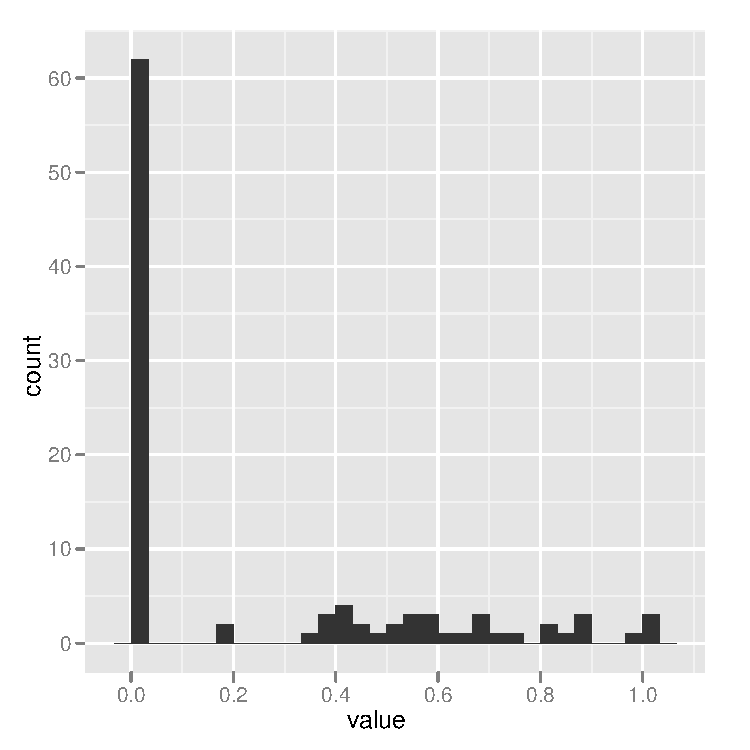
\includegraphics{Fig1a} 

\end{kframe}}
\end{knitrout}

\end{center}
\label{fig:onea}
\end{figure}

Note that the ability to estimate lambda is very poor, with most simulations returning an estimate of almost zero despite the true value used in the simulations being .  Estimating the sigma parameter is somewhat more reliable, even on this small tree:

\setkeys{Gin}{width=0.45\textwidth}
\begin{figure}
\begin{center}
\begin{knitrout}
\definecolor{shadecolor}{rgb}{.97, .97, .97}{\color{fgcolor}\begin{kframe}
\begin{flushleft}
\ttfamily\noindent
\hlsymbol{betas}{\ }\hlassignement{\usebox{\hlnormalsizeboxlessthan}-}{\ }\hlfunctioncall{subset}\hlkeyword{(}\hlsymbol{bm\usebox{\hlnormalsizeboxunderscore}v\usebox{\hlnormalsizeboxunderscore}lambda}\hlkeyword{[[}\hlstring{"{}par\usebox{\hlnormalsizeboxunderscore}dists"{}}\hlkeyword{]}\hlkeyword{]}\hlkeyword{,}{\ }\hlsymbol{comparison}{\ }==\hspace*{\fill}\\
\hlstd{}{\ }{\ }{\ }{\ }\hlstring{"{}BB"{}}{\ }\hlkeyword{\usebox{\hlnormalsizeboxand}}{\ }\hlsymbol{parameter}{\ }=={\ }\hlstring{"{}beta"{}}\hlkeyword{)}\hspace*{\fill}\\
\hlstd{}\hlsymbol{p2}{\ }\hlassignement{\usebox{\hlnormalsizeboxlessthan}-}{\ }\hlfunctioncall{ggplot}\hlkeyword{(}\hlsymbol{betas}\hlkeyword{)}{\ }\hlkeyword{+}{\ }\hlfunctioncall{geom\usebox{\hlnormalsizeboxunderscore}histogram}\hlkeyword{(}\hlfunctioncall{aes}\hlkeyword{(}\hlfunctioncall{sqrt}\hlkeyword{(}\hlsymbol{value}\hlkeyword{)}\hlkeyword{)}\hlkeyword{)}{\ }{\ }\hlcomment{\usebox{\hlnormalsizeboxhash}{\ }beta{\ }=={\ }sigma\usebox{\hlnormalsizeboxhat}2}\hspace*{\fill}\\
\hlstd{}\hlfunctioncall{print}\hlkeyword{(}\hlsymbol{p2}\hlkeyword{)}\mbox{}
\normalfont
\end{flushleft}


\centering{}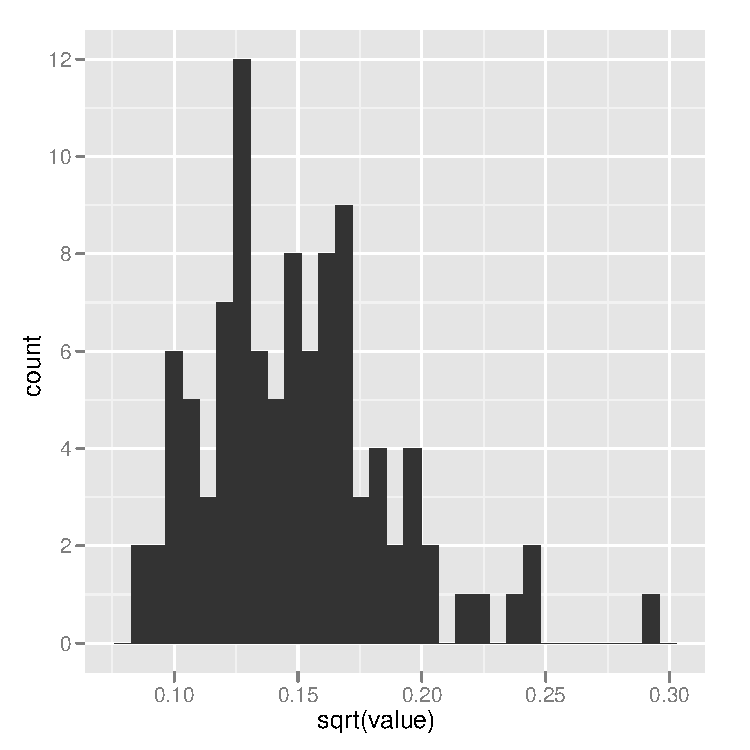
\includegraphics{Fig1b} 

\end{kframe}}
\end{knitrout}

\end{center}
\label{fig:oneb}
\end{figure}


We can also query the confidence intervals directly from the estimates returned by the pmc function.  Using the lambda value we already extracted, we can get confidence intervals, 

\begin{knitrout}
\definecolor{shadecolor}{rgb}{.97, .97, .97}{\color{fgcolor}\begin{kframe}
\begin{flushleft}
\ttfamily\noindent
\hlfunctioncall{cast}\hlkeyword{(}\hlsymbol{lambdas}\hlkeyword{,}{\ }\hlsymbol{comparison}{\ }\hlkeyword{\urltilda{}}{\ }\hlsymbol{parameter}\hlkeyword{,}{\ }\hlkeyword{function}\hlkeyword{(}\hlformalargs{x}\hlkeyword{)}{\ }\hlfunctioncall{quantile}\hlkeyword{(}\hlsymbol{x}\hlkeyword{,}\hspace*{\fill}\\
\hlstd{}{\ }{\ }{\ }{\ }\hlfunctioncall{c}\hlkeyword{(}\hlnumber{0.05}\hlkeyword{,}{\ }\hlnumber{0.95}\hlkeyword{)}\hlkeyword{)}\hlkeyword{,}{\ }\hlargument{value}{\ }\hlargument{=}{\ }\hlfunctioncall{c}\hlkeyword{(}\hlstring{"{}lower"{}}\hlkeyword{,}{\ }\hlstring{"{}upper"{}}\hlkeyword{)}\hlkeyword{)}\mbox{}
\normalfont
\end{flushleft}
\begin{verbatim}
##   comparison lambda_X5. lambda_X95.
## 1         BB      1e-07      0.8914
\end{verbatim}
\end{kframe}}
\end{knitrout}


Or get the intervals for all parameters at once. Note that the ``comparison'' indicates the model being fit with the first letter, and the model used for the simulations under the second letter. 
\begin{knitrout}
\definecolor{shadecolor}{rgb}{.97, .97, .97}{\color{fgcolor}\begin{kframe}
\begin{flushleft}
\ttfamily\noindent
\hlfunctioncall{cast}\hlkeyword{(}\hlsymbol{bm\usebox{\hlnormalsizeboxunderscore}v\usebox{\hlnormalsizeboxunderscore}lambda}\hlkeyword{\usebox{\hlnormalsizeboxdollar}}\hlsymbol{par\usebox{\hlnormalsizeboxunderscore}dist}\hlkeyword{,}{\ }\hlsymbol{comparison}{\ }\hlkeyword{\urltilda{}}{\ }\hlsymbol{parameter}\hlkeyword{,}\hspace*{\fill}\\
\hlstd{}{\ }{\ }{\ }{\ }\hlkeyword{function}\hlkeyword{(}\hlformalargs{x}\hlkeyword{)}{\ }\hlfunctioncall{quantile}\hlkeyword{(}\hlsymbol{x}\hlkeyword{,}{\ }\hlfunctioncall{c}\hlkeyword{(}\hlnumber{0.05}\hlkeyword{,}{\ }\hlnumber{0.95}\hlkeyword{)}\hlkeyword{)}\hlkeyword{,}{\ }\hlargument{value}{\ }\hlargument{=}{\ }\hlfunctioncall{c}\hlkeyword{(}\hlstring{"{}lower"{}}\hlkeyword{,}\hspace*{\fill}\\
\hlstd{}{\ }{\ }{\ }{\ }{\ }{\ }{\ }{\ }\hlstring{"{}upper"{}}\hlkeyword{)}\hlkeyword{)}\mbox{}
\normalfont
\end{flushleft}
\begin{verbatim}
##   comparison beta_X5. beta_X95. k_X5. k_X95. lambda_X5. lambda_X95.
## 1         AA 0.050629   0.81811     2      2         NA          NA
## 2         AB 0.030543   0.29036     2      2         NA          NA
## 3         BA 0.013356   0.09850     3      3      1e-07      0.9733
## 4         BB 0.009438   0.04731     3      3      1e-07      0.8914
##   lnl_X5. lnl_X95.  lr_X5. lr_X95. root_X5. root_X95.
## 1 -7.6841    10.40 -7.6841   10.40    4.107     4.395
## 2 -0.9532    13.68 -0.9532   13.68    4.166     4.355
## 3  1.7368    13.74  1.7368   13.74    4.073     4.423
## 4  6.6146    15.85  6.6146   15.85    4.160     4.367
\end{verbatim}
\end{kframe}}
\end{knitrout}

This way we can see the interval for lambda estimated when simulating under the brownian motion model (equiv to lambda=1) under the row BA, as well as the confidence interval on the lambda estimate when simulating with the correct model, lambda=0.6. These cross-comparisons can also be useful. We could always use variations of the subset command above to include only certain parameters or comparisons. We can also summarize all this information at once in a traditional box-and-whiskers plot, Fig~\ref{fig:pars}.  We can repeat the analysis with a larger tree, showing the uncertainty in the estimate of lambda decreases, if only slowly, Fig~\ref{fig:onec}.
\setkeys{Gin}{width=0.85\textwidth}
\begin{figure}
\begin{center}
\begin{knitrout}
\definecolor{shadecolor}{rgb}{.97, .97, .97}{\color{fgcolor}\begin{kframe}
\begin{flushleft}
\ttfamily\noindent
\hlsymbol{p3}{\ }\hlassignement{\usebox{\hlnormalsizeboxlessthan}-}{\ }\hlfunctioncall{plot\usebox{\hlnormalsizeboxunderscore}pars}\hlkeyword{(}\hlsymbol{bm\usebox{\hlnormalsizeboxunderscore}v\usebox{\hlnormalsizeboxunderscore}lambda}\hlkeyword{\usebox{\hlnormalsizeboxdollar}}\hlsymbol{par\usebox{\hlnormalsizeboxunderscore}dists}\hlkeyword{)}\hspace*{\fill}\\
\hlstd{}\hlfunctioncall{print}\hlkeyword{(}\hlsymbol{p3}\hlkeyword{)}\mbox{}
\normalfont
\end{flushleft}


\centering{}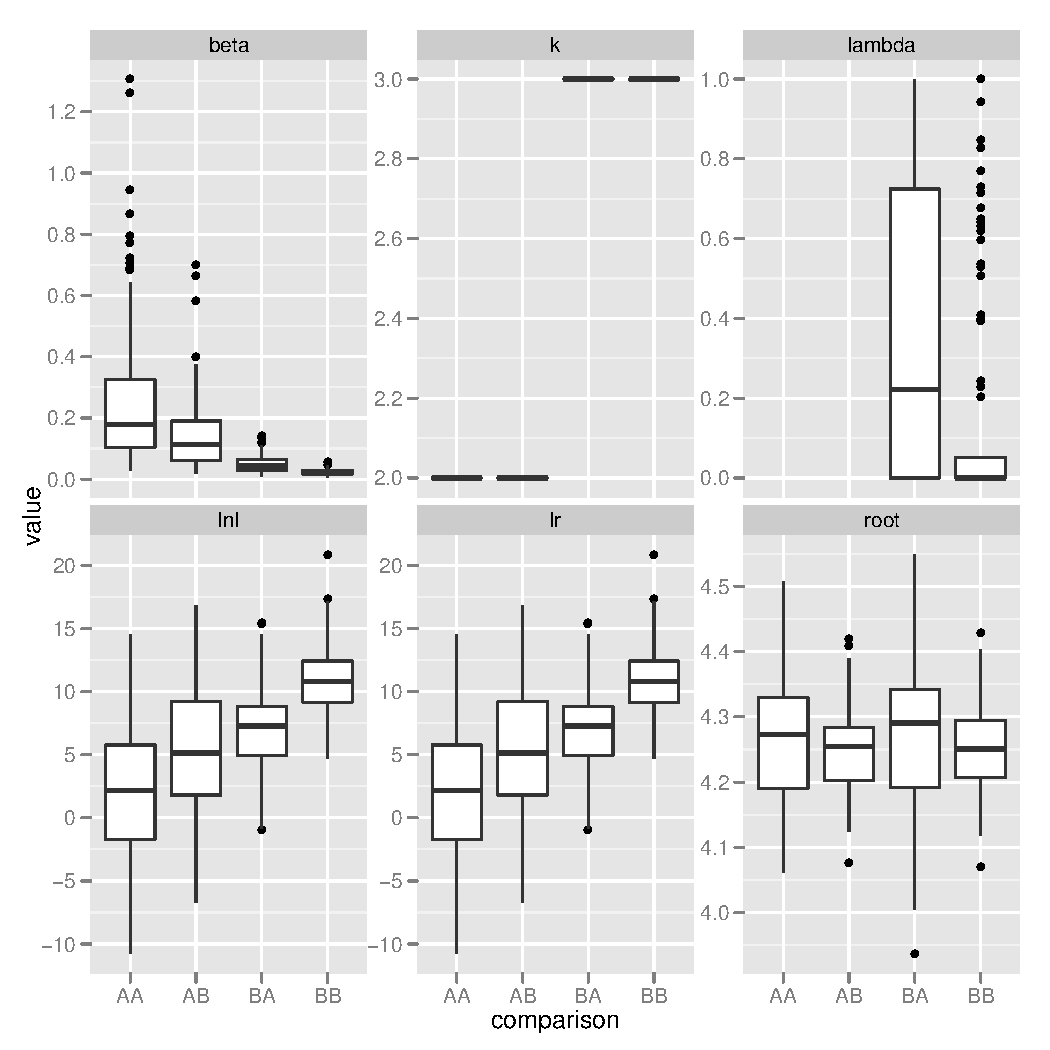
\includegraphics{allpars} 

\end{kframe}}
\end{knitrout}

\end{center}
\label{fig:pars}
\end{figure}


% needed on linux machines to avoid stupid errors from treesim/droptip


\setkeys{Gin}{width=0.45\textwidth}



\begin{knitrout}
\definecolor{shadecolor}{rgb}{.97, .97, .97}{\color{fgcolor}\begin{kframe}
\begin{flushleft}
\ttfamily\noindent
\hlfunctioncall{require}\hlkeyword{(}\hlsymbol{TreeSim}\hlkeyword{)}\hspace*{\fill}\\
\hlstd{}\hlsymbol{simtree}{\ }\hlassignement{\usebox{\hlnormalsizeboxlessthan}-}{\ }\hlfunctioncall{sim.bd.taxa}\hlkeyword{(}\hlargument{n}{\ }\hlargument{=}{\ }\hlnumber{281}\hlkeyword{,}{\ }\hlargument{numbsim}{\ }\hlargument{=}{\ }\hlnumber{1}\hlkeyword{,}{\ }\hlargument{lambda}{\ }\hlargument{=}{\ }\hlnumber{1}\hlkeyword{,}\hspace*{\fill}\\
\hlstd{}{\ }{\ }{\ }{\ }\hlargument{mu}{\ }\hlargument{=}{\ }\hlnumber{0}\hlkeyword{,}{\ }\hlargument{frac}{\ }\hlargument{=}{\ }\hlnumber{1}\hlkeyword{,}{\ }\hlargument{complete}{\ }\hlargument{=}{\ }\hlnumber{FALSE}\hlkeyword{,}{\ }\hlargument{stochsampling}{\ }\hlargument{=}{\ }\hlnumber{FALSE}\hlkeyword{)}\hlkeyword{[[}\hlnumber{1}\hlkeyword{]}\hlkeyword{]}\hlkeyword{[[}\hlnumber{1}\hlkeyword{]}\hlkeyword{]}\hspace*{\fill}\\
\hlstd{}\hlsymbol{simdat}{\ }\hlassignement{\usebox{\hlnormalsizeboxlessthan}-}{\ }\hlfunctioncall{rTraitCont}\hlkeyword{(}\hlfunctioncall{lambdaTree}\hlkeyword{(}\hlsymbol{simtree}\hlkeyword{,}{\ }\hlnumber{0.6}\hlkeyword{)}\hlkeyword{,}\hspace*{\fill}\\
\hlstd{}{\ }{\ }{\ }{\ }\hlargument{sigma}{\ }\hlargument{=}{\ }\hlnumber{2}\hlkeyword{)}\hspace*{\fill}\\
\hlstd{}\hlsymbol{bm\usebox{\hlnormalsizeboxunderscore}v\usebox{\hlnormalsizeboxunderscore}lambda}{\ }\hlassignement{\usebox{\hlnormalsizeboxlessthan}-}{\ }\hlfunctioncall{pmc}\hlkeyword{(}\hlsymbol{simtree}\hlkeyword{,}{\ }\hlsymbol{simdat}\hlkeyword{,}{\ }\hlstring{"{}BM"{}}\hlkeyword{,}{\ }\hlstring{"{}lambda"{}}\hlkeyword{,}\hspace*{\fill}\\
\hlstd{}{\ }{\ }{\ }{\ }\hlargument{nboot}{\ }\hlargument{=}{\ }\hlnumber{20}\hlkeyword{)}\mbox{}
\normalfont
\end{flushleft}
\end{kframe}}
\end{knitrout}


\begin{figure}
\begin{center}
\begin{knitrout}
\definecolor{shadecolor}{rgb}{.97, .97, .97}{\color{fgcolor}\begin{kframe}
\begin{flushleft}
\ttfamily\noindent
\hlsymbol{lambdas}{\ }\hlassignement{\usebox{\hlnormalsizeboxlessthan}-}{\ }\hlfunctioncall{subset}\hlkeyword{(}\hlsymbol{bm\usebox{\hlnormalsizeboxunderscore}v\usebox{\hlnormalsizeboxunderscore}lambda}\hlkeyword{[[}\hlstring{"{}par\usebox{\hlnormalsizeboxunderscore}dists"{}}\hlkeyword{]}\hlkeyword{]}\hlkeyword{,}\hspace*{\fill}\\
\hlstd{}{\ }{\ }{\ }{\ }\hlsymbol{comparison}{\ }=={\ }\hlstring{"{}BB"{}}{\ }\hlkeyword{\usebox{\hlnormalsizeboxand}}{\ }\hlsymbol{parameter}{\ }=={\ }\hlstring{"{}lambda"{}}\hlkeyword{)}\hspace*{\fill}\\
\hlstd{}\hlsymbol{p4}{\ }\hlassignement{\usebox{\hlnormalsizeboxlessthan}-}{\ }\hlfunctioncall{ggplot}\hlkeyword{(}\hlsymbol{lambdas}\hlkeyword{)}{\ }\hlkeyword{+}{\ }\hlfunctioncall{geom\usebox{\hlnormalsizeboxunderscore}histogram}\hlkeyword{(}\hlfunctioncall{aes}\hlkeyword{(}\hlsymbol{value}\hlkeyword{)}\hlkeyword{)}{\ }\hlkeyword{+}\hspace*{\fill}\\
\hlstd{}{\ }{\ }{\ }{\ }\hlfunctioncall{geom\usebox{\hlnormalsizeboxunderscore}vline}\hlkeyword{(}\hlargument{xintercept}{\ }\hlargument{=}{\ }\hlsymbol{bm\usebox{\hlnormalsizeboxunderscore}v\usebox{\hlnormalsizeboxunderscore}lambda}\hlkeyword{[[}\hlstring{"{}B"{}}\hlkeyword{]}\hlkeyword{]}\hlkeyword{[[}\hlstring{"{}wingL"{}}\hlkeyword{]}\hlkeyword{]}\hlkeyword{[[}\hlstring{"{}lambda"{}}\hlkeyword{]}\hlkeyword{]}\hlkeyword{)}\hspace*{\fill}\\
\hlstd{}\hlfunctioncall{print}\hlkeyword{(}\hlsymbol{p4}\hlkeyword{)}\mbox{}
\normalfont
\end{flushleft}
\end{kframe}}
\end{knitrout}

\end{center}
\label{fig:onec}
\end{figure}

\section{Anoles example}
Next we consider the examples re-analyzing the Anoles data from~\citep{Butler2004}, using methods from the ouch package.  
\begin{knitrout}
\definecolor{shadecolor}{rgb}{.97, .97, .97}{\color{fgcolor}\begin{kframe}
\begin{flushleft}
\ttfamily\noindent
\hlfunctioncall{data}\hlkeyword{(}\hlsymbol{anoles}\hlkeyword{)}\hspace*{\fill}\\
\hlstd{}\hlsymbol{ou3v4}{\ }\hlassignement{\usebox{\hlnormalsizeboxlessthan}-}{\ }\hlfunctioncall{pmc}\hlkeyword{(}\hlsymbol{tree}\hlkeyword{,}{\ }\hlfunctioncall{log}\hlkeyword{(}\hlsymbol{anoles}\hlkeyword{[}\hlstring{"{}size"{}}\hlkeyword{]}\hlkeyword{)}\hlkeyword{,}{\ }\hlargument{modelA}{\ }\hlargument{=}{\ }\hlstring{"{}hansen"{}}\hlkeyword{,}\hspace*{\fill}\\
\hlstd{}{\ }{\ }{\ }{\ }\hlargument{modelB}{\ }\hlargument{=}{\ }\hlstring{"{}hansen"{}}\hlkeyword{,}{\ }\hlargument{optionsA}{\ }\hlargument{=}{\ }\hlfunctioncall{list}\hlkeyword{(}\hlargument{regimes}{\ }\hlargument{=}{\ }\hlsymbol{anoles}\hlkeyword{[}\hlstring{"{}OU.LP"{}}\hlkeyword{]}\hlkeyword{,}\hspace*{\fill}\\
\hlstd{}{\ }{\ }{\ }{\ }{\ }{\ }{\ }{\ }\hlargument{sqrt.alpha}{\ }\hlargument{=}{\ }\hlnumber{1}\hlkeyword{,}{\ }\hlargument{sigma}{\ }\hlargument{=}{\ }\hlnumber{1}\hlkeyword{)}\hlkeyword{,}{\ }\hlargument{optionsB}{\ }\hlargument{=}{\ }\hlfunctioncall{list}\hlkeyword{(}\hlargument{regimes}{\ }\hlargument{=}{\ }\hlsymbol{anoles}\hlkeyword{[}\hlstring{"{}OU.4"{}}\hlkeyword{]}\hlkeyword{,}\hspace*{\fill}\\
\hlstd{}{\ }{\ }{\ }{\ }{\ }{\ }{\ }{\ }\hlargument{sqrt.alpha}{\ }\hlargument{=}{\ }\hlnumber{1}\hlkeyword{,}{\ }\hlargument{sigma}{\ }\hlargument{=}{\ }\hlnumber{1}\hlkeyword{)}\hlkeyword{,}{\ }\hlargument{nboot}{\ }\hlargument{=}{\ }\hlnumber{100}\hlkeyword{)}\hspace*{\fill}\\
\hlstd{}\hspace*{\fill}\\
\hlstd{}\hlsymbol{ou3v15}{\ }\hlassignement{\usebox{\hlnormalsizeboxlessthan}-}{\ }\hlfunctioncall{pmc}\hlkeyword{(}\hlsymbol{tree}\hlkeyword{,}{\ }\hlfunctioncall{log}\hlkeyword{(}\hlsymbol{anoles}\hlkeyword{[}\hlstring{"{}size"{}}\hlkeyword{]}\hlkeyword{)}\hlkeyword{,}{\ }\hlstring{"{}hansen"{}}\hlkeyword{,}\hspace*{\fill}\\
\hlstd{}{\ }{\ }{\ }{\ }\hlstring{"{}hansen"{}}\hlkeyword{,}{\ }\hlfunctioncall{list}\hlkeyword{(}\hlargument{regimes}{\ }\hlargument{=}{\ }\hlsymbol{anoles}\hlkeyword{[}\hlstring{"{}OU.LP"{}}\hlkeyword{]}\hlkeyword{,}{\ }\hlargument{sqrt.alpha}{\ }\hlargument{=}{\ }\hlnumber{1}\hlkeyword{,}\hspace*{\fill}\\
\hlstd{}{\ }{\ }{\ }{\ }{\ }{\ }{\ }{\ }\hlargument{sigma}{\ }\hlargument{=}{\ }\hlnumber{1}\hlkeyword{)}\hlkeyword{,}{\ }\hlfunctioncall{list}\hlkeyword{(}\hlargument{regimes}{\ }\hlargument{=}{\ }\hlsymbol{anoles}\hlkeyword{[}\hlstring{"{}OU.15"{}}\hlkeyword{]}\hlkeyword{,}{\ }\hlargument{sqrt.alpha}{\ }\hlargument{=}{\ }\hlnumber{1}\hlkeyword{,}\hspace*{\fill}\\
\hlstd{}{\ }{\ }{\ }{\ }{\ }{\ }{\ }{\ }\hlargument{sigma}{\ }\hlargument{=}{\ }\hlnumber{1}\hlkeyword{)}\hlkeyword{,}{\ }\hlargument{nboot}{\ }\hlargument{=}{\ }\hlnumber{100}\hlkeyword{)}\hspace*{\fill}\\
\hlstd{}\hspace*{\fill}\\
\hlstd{}\hlsymbol{ou1v3}{\ }\hlassignement{\usebox{\hlnormalsizeboxlessthan}-}{\ }\hlfunctioncall{pmc}\hlkeyword{(}\hlsymbol{tree}\hlkeyword{,}{\ }\hlfunctioncall{log}\hlkeyword{(}\hlsymbol{anoles}\hlkeyword{[}\hlstring{"{}size"{}}\hlkeyword{]}\hlkeyword{)}\hlkeyword{,}{\ }\hlstring{"{}hansen"{}}\hlkeyword{,}\hspace*{\fill}\\
\hlstd{}{\ }{\ }{\ }{\ }\hlstring{"{}hansen"{}}\hlkeyword{,}{\ }\hlfunctioncall{list}\hlkeyword{(}\hlargument{regimes}{\ }\hlargument{=}{\ }\hlsymbol{anoles}\hlkeyword{[}\hlstring{"{}OU.1"{}}\hlkeyword{]}\hlkeyword{,}{\ }\hlargument{sqrt.alpha}{\ }\hlargument{=}{\ }\hlnumber{1}\hlkeyword{,}\hspace*{\fill}\\
\hlstd{}{\ }{\ }{\ }{\ }{\ }{\ }{\ }{\ }\hlargument{sigma}{\ }\hlargument{=}{\ }\hlnumber{1}\hlkeyword{)}\hlkeyword{,}{\ }\hlfunctioncall{list}\hlkeyword{(}\hlargument{regimes}{\ }\hlargument{=}{\ }\hlsymbol{anoles}\hlkeyword{[}\hlstring{"{}OU.LP"{}}\hlkeyword{]}\hlkeyword{,}{\ }\hlargument{sqrt.alpha}{\ }\hlargument{=}{\ }\hlnumber{1}\hlkeyword{,}\hspace*{\fill}\\
\hlstd{}{\ }{\ }{\ }{\ }{\ }{\ }{\ }{\ }\hlargument{sigma}{\ }\hlargument{=}{\ }\hlnumber{1}\hlkeyword{)}\hlkeyword{,}{\ }\hlargument{nboot}{\ }\hlargument{=}{\ }\hlnumber{100}\hlkeyword{)}\hspace*{\fill}\\
\hlstd{}\hspace*{\fill}\\
\hlstd{}\hlsymbol{ou0v1}{\ }\hlassignement{\usebox{\hlnormalsizeboxlessthan}-}{\ }\hlfunctioncall{pmc}\hlkeyword{(}\hlsymbol{tree}\hlkeyword{,}{\ }\hlfunctioncall{log}\hlkeyword{(}\hlsymbol{anoles}\hlkeyword{[}\hlstring{"{}size"{}}\hlkeyword{]}\hlkeyword{)}\hlkeyword{,}{\ }\hlstring{"{}brown"{}}\hlkeyword{,}\hspace*{\fill}\\
\hlstd{}{\ }{\ }{\ }{\ }\hlstring{"{}hansen"{}}\hlkeyword{,}{\ }\hlfunctioncall{list}\hlkeyword{(}\hlkeyword{)}\hlkeyword{,}{\ }\hlfunctioncall{list}\hlkeyword{(}\hlargument{regimes}{\ }\hlargument{=}{\ }\hlsymbol{anoles}\hlkeyword{[}\hlstring{"{}OU.1"{}}\hlkeyword{]}\hlkeyword{,}{\ }\hlargument{sqrt.alpha}{\ }\hlargument{=}{\ }\hlnumber{1}\hlkeyword{,}\hspace*{\fill}\\
\hlstd{}{\ }{\ }{\ }{\ }{\ }{\ }{\ }{\ }\hlargument{sigma}{\ }\hlargument{=}{\ }\hlnumber{1}\hlkeyword{)}\hlkeyword{,}{\ }\hlargument{nboot}{\ }\hlargument{=}{\ }\hlnumber{100}\hlkeyword{)}\mbox{}
\normalfont
\end{flushleft}
\end{kframe}}
\end{knitrout}



\setkeys{Gin}{width=\textwidth}
\begin{figure}
\begin{center}
\begin{knitrout}
\definecolor{shadecolor}{rgb}{.97, .97, .97}{\color{fgcolor}\begin{kframe}
\begin{flushleft}
\ttfamily\noindent
\hlsymbol{a}{\ }\hlassignement{\usebox{\hlnormalsizeboxlessthan}-}{\ }\hlfunctioncall{plot}\hlkeyword{(}\hlsymbol{ou3v4}\hlkeyword{,}{\ }\hlargument{A}{\ }\hlargument{=}{\ }\hlstring{"{}OU.3"{}}\hlkeyword{,}{\ }\hlargument{B}{\ }\hlargument{=}{\ }\hlstring{"{}OU.4"{}}\hlkeyword{)}\hspace*{\fill}\\
\hlstd{}\hlsymbol{b}{\ }\hlassignement{\usebox{\hlnormalsizeboxlessthan}-}{\ }\hlfunctioncall{plot}\hlkeyword{(}\hlsymbol{ou3v15}\hlkeyword{,}{\ }\hlargument{A}{\ }\hlargument{=}{\ }\hlstring{"{}OU.3"{}}\hlkeyword{,}{\ }\hlargument{B}{\ }\hlargument{=}{\ }\hlstring{"{}OU.15"{}}\hlkeyword{)}\hspace*{\fill}\\
\hlstd{}\hlsymbol{c}{\ }\hlassignement{\usebox{\hlnormalsizeboxlessthan}-}{\ }\hlfunctioncall{plot}\hlkeyword{(}\hlsymbol{ou1v3}\hlkeyword{,}{\ }\hlargument{A}{\ }\hlargument{=}{\ }\hlstring{"{}OU.1"{}}\hlkeyword{,}{\ }\hlargument{B}{\ }\hlargument{=}{\ }\hlstring{"{}OU.3"{}}\hlkeyword{)}\hspace*{\fill}\\
\hlstd{}\hlsymbol{d}{\ }\hlassignement{\usebox{\hlnormalsizeboxlessthan}-}{\ }\hlfunctioncall{plot}\hlkeyword{(}\hlsymbol{ou0v1}\hlkeyword{,}{\ }\hlargument{A}{\ }\hlargument{=}{\ }\hlstring{"{}BM"{}}\hlkeyword{,}{\ }\hlargument{B}{\ }\hlargument{=}{\ }\hlstring{"{}OU.1"{}}\hlkeyword{)}\hspace*{\fill}\\
\hlstd{}\hspace*{\fill}\\
\hlstd{}\hlfunctioncall{grid.newpage}\hlkeyword{(}\hlkeyword{)}\hspace*{\fill}\\
\hlstd{}\hlfunctioncall{pushViewport}\hlkeyword{(}\hlfunctioncall{viewport}\hlkeyword{(}\hlargument{layout}{\ }\hlargument{=}{\ }\hlfunctioncall{grid.layout}\hlkeyword{(}\hlnumber{2}\hlkeyword{,}\hspace*{\fill}\\
\hlstd{}{\ }{\ }{\ }{\ }\hlnumber{2}\hlkeyword{)}\hlkeyword{)}\hlkeyword{)}\hspace*{\fill}\\
\hlstd{}\hlsymbol{vplayout}{\ }\hlassignement{\usebox{\hlnormalsizeboxlessthan}-}{\ }\hlkeyword{function}\hlkeyword{(}\hlformalargs{x}\hlkeyword{,}{\ }\hlformalargs{y}\hlkeyword{)}{\ }\hlfunctioncall{viewport}\hlkeyword{(}\hlargument{layout.pos.row}{\ }\hlargument{=}{\ }\hlsymbol{x}\hlkeyword{,}\hspace*{\fill}\\
\hlstd{}{\ }{\ }{\ }{\ }\hlargument{layout.pos.col}{\ }\hlargument{=}{\ }\hlsymbol{y}\hlkeyword{)}\hspace*{\fill}\\
\hlstd{}\hlfunctioncall{print}\hlkeyword{(}\hlsymbol{a}\hlkeyword{,}{\ }\hlargument{vp}{\ }\hlargument{=}{\ }\hlfunctioncall{vplayout}\hlkeyword{(}\hlnumber{1}\hlkeyword{,}{\ }\hlnumber{1}\hlkeyword{)}\hlkeyword{)}\hspace*{\fill}\\
\hlstd{}\hlfunctioncall{print}\hlkeyword{(}\hlsymbol{b}\hlkeyword{,}{\ }\hlargument{vp}{\ }\hlargument{=}{\ }\hlfunctioncall{vplayout}\hlkeyword{(}\hlnumber{1}\hlkeyword{,}{\ }\hlnumber{2}\hlkeyword{)}\hlkeyword{)}\hspace*{\fill}\\
\hlstd{}\hlfunctioncall{print}\hlkeyword{(}\hlsymbol{c}\hlkeyword{,}{\ }\hlargument{vp}{\ }\hlargument{=}{\ }\hlfunctioncall{vplayout}\hlkeyword{(}\hlnumber{2}\hlkeyword{,}{\ }\hlnumber{1}\hlkeyword{)}\hlkeyword{)}\hspace*{\fill}\\
\hlstd{}\hlfunctioncall{print}\hlkeyword{(}\hlsymbol{d}\hlkeyword{,}{\ }\hlargument{vp}{\ }\hlargument{=}{\ }\hlfunctioncall{vplayout}\hlkeyword{(}\hlnumber{2}\hlkeyword{,}{\ }\hlnumber{2}\hlkeyword{)}\hlkeyword{)}\mbox{}
\normalfont
\end{flushleft}


\centering{}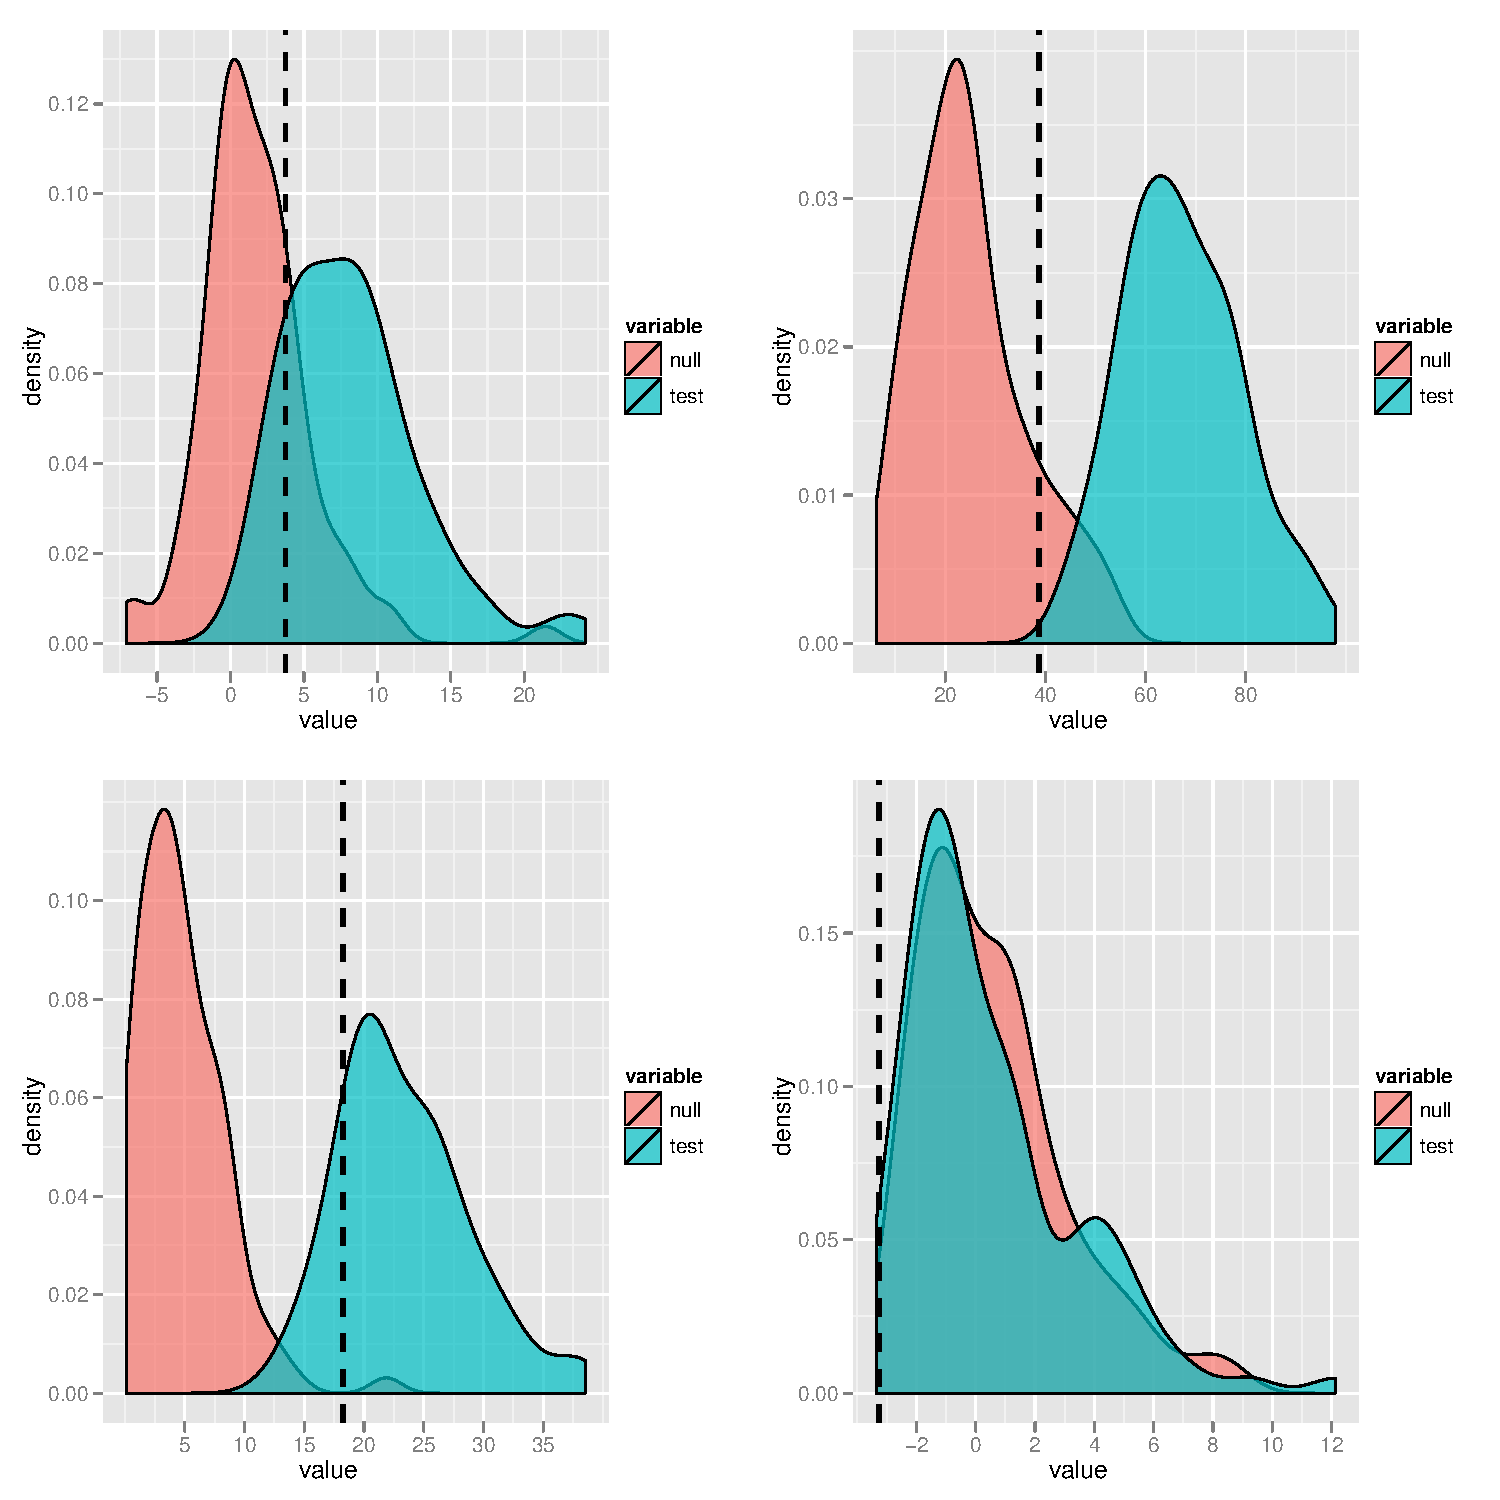
\includegraphics{plot_anoles} 

\end{kframe}}
\end{knitrout}

\end{center}
\end{figure}


Fits from the ouch methods include a phylogeny in the ouch format.  As many researchers would rather manipulate and plot the resulting phylogeny in the "phylo" format from the ape package, pmc provides a simple utility to convert the tree while keeping track of the regimes in ouch.  \footnote{Some caution should always be applied in using "phylo" format trees.  Unlike the ouch format, a given tree does not have a unique specification, and consequently some functions that use "phylo" trees make assumptions about the ordering of edges that may not be true, even for a technically valid, plottable "phylo" specification of the phylogeny.}
%\begin{figure}
%\begin{center}
%<<treeplotting>>=
%require(ape)
%## Convert is a custom pmc function that toggles between tree formats
%ou4_tree <- convert(tree, regimes=anoles[["OU.4"]])
%plot(ou4_tree, edge.color = treepalette(ou4_tree), edge.width=5, cex=1.2, show.tip.label=TRUE)
%mtext("OU.4 regimes", cex=2)
%@
%\end{center}
%\end{figure}
%

\section{Early Burst models}
We can also mix and match methods, comparing a fit from geiger with a fit from ouch.  We do so in this example, which shows that it may be very difficult to identify if a given dataset comes from an early burst or a OU model, Fig~\ref{fig:eb}.




\begin{knitrout}
\definecolor{shadecolor}{rgb}{.97, .97, .97}{\color{fgcolor}\begin{kframe}
\begin{flushleft}
\ttfamily\noindent
\hlfunctioncall{require}\hlkeyword{(}\hlsymbol{pmc}\hlkeyword{)}\hspace*{\fill}\\
\hlstd{}\hlfunctioncall{require}\hlkeyword{(}\hlsymbol{TreeSim}\hlkeyword{)}{\ }\hlcomment{\usebox{\hlnormalsizeboxhash}{\ }to{\ }simulate{\ }a{\ }sample{\ }phyologeny}\hspace*{\fill}\\
\hlstd{}\hlsymbol{simtree}{\ }\hlassignement{\usebox{\hlnormalsizeboxlessthan}-}{\ }\hlfunctioncall{sim.bd.taxa}\hlkeyword{(}\hlargument{n}\hlargument{=}\hlnumber{60}\hlkeyword{,}{\ }\hlargument{numbsim}\hlargument{=}\hlnumber{1}\hlkeyword{,}{\ }\hlargument{lambda}\hlargument{=}\hlnumber{1}\hlkeyword{,}{\ }\hlargument{mu}\hlargument{=}\hlnumber{0}\hlkeyword{,}{\ }\hlargument{frac}\hlargument{=}\hlnumber{1}\hlkeyword{,}\hspace*{\fill}\\
\hlstd{}{\ }{\ }{\ }{\ }{\ }{\ }{\ }{\ }{\ }{\ }{\ }{\ }{\ }{\ }{\ }{\ }{\ }{\ }{\ }{\ }{\ }{\ }{\ }\hlargument{complete}\hlargument{=}\hlnumber{FALSE}\hlkeyword{,}{\ }\hlargument{stochsampling}\hlargument{=}\hlnumber{FALSE}\hlkeyword{)}\hlkeyword{[[}\hlnumber{1}\hlkeyword{]}\hlkeyword{]}\hlkeyword{[[}\hlnumber{1}\hlkeyword{]}\hlkeyword{]}\hspace*{\fill}\\
\hlstd{}\hlsymbol{dat}{\ }\hlassignement{\usebox{\hlnormalsizeboxlessthan}-}{\ }\hlfunctioncall{rTraitCont}\hlkeyword{(}\hlfunctioncall{exponentialchangeTree}\hlkeyword{(}\hlsymbol{simtree}\hlkeyword{,}{\ }\hlargument{a}\hlargument{=}\hlkeyword{-}\hlnumber{0.5}\hlkeyword{)}\hlkeyword{,}{\ }\hlargument{sigma}\hlargument{=}\hlnumber{5}\hlkeyword{)}\hspace*{\fill}\\
\hlstd{}\hlsymbol{regimes}{\ }\hlassignement{\usebox{\hlnormalsizeboxlessthan}-}{\ }\hlfunctioncall{format\usebox{\hlnormalsizeboxunderscore}data}\hlkeyword{(}\hlsymbol{simtree}\hlkeyword{,}\hlsymbol{dat}\hlkeyword{)}\hlkeyword{\usebox{\hlnormalsizeboxdollar}}\hlsymbol{noregimes}\hspace*{\fill}\\
\hlstd{}{\ }{\ }\hlsymbol{eb\usebox{\hlnormalsizeboxunderscore}v\usebox{\hlnormalsizeboxunderscore}ou}{\ }\hlassignement{\usebox{\hlnormalsizeboxlessthan}-}{\ }\hlfunctioncall{pmc}\hlkeyword{(}\hlsymbol{simtree}\hlkeyword{,}{\ }\hlsymbol{dat}\hlkeyword{,}{\ }\hlargument{modelA}{\ }\hlargument{=}{\ }\hlstring{"{}EB"{}}\hlkeyword{,}{\ }\hlargument{modelB}{\ }\hlargument{=}{\ }\hlstring{"{}hansen"{}}\hlkeyword{,}\hspace*{\fill}\\
\hlstd{}{\ }{\ }{\ }{\ }\hlargument{optionsB}{\ }\hlargument{=}{\ }\hlfunctioncall{list}\hlkeyword{(}\hlargument{sqrt.alpha}{\ }\hlargument{=}{\ }\hlnumber{1}\hlkeyword{,}{\ }\hlargument{sigma}{\ }\hlargument{=}{\ }\hlnumber{1}\hlkeyword{,}{\ }\hlargument{regimes}{\ }\hlargument{=}{\ }\hlsymbol{regimes}\hlkeyword{)}\hlkeyword{,}\hspace*{\fill}\\
\hlstd{}{\ }{\ }{\ }{\ }\hlargument{nboot}{\ }\hlargument{=}{\ }\hlnumber{50}\hlkeyword{)}\mbox{}
\normalfont
\end{flushleft}
\end{kframe}}
\end{knitrout}



\setkeys{Gin}{width=.5\textwidth}
\begin{figure}
\begin{knitrout}
\definecolor{shadecolor}{rgb}{.97, .97, .97}{\color{fgcolor}\begin{kframe}
\begin{flushleft}
\ttfamily\noindent
\hlfunctioncall{plot}\hlkeyword{(}\hlsymbol{eb\usebox{\hlnormalsizeboxunderscore}v\usebox{\hlnormalsizeboxunderscore}ou}\hlkeyword{)}\mbox{}
\normalfont
\end{flushleft}


\centering{}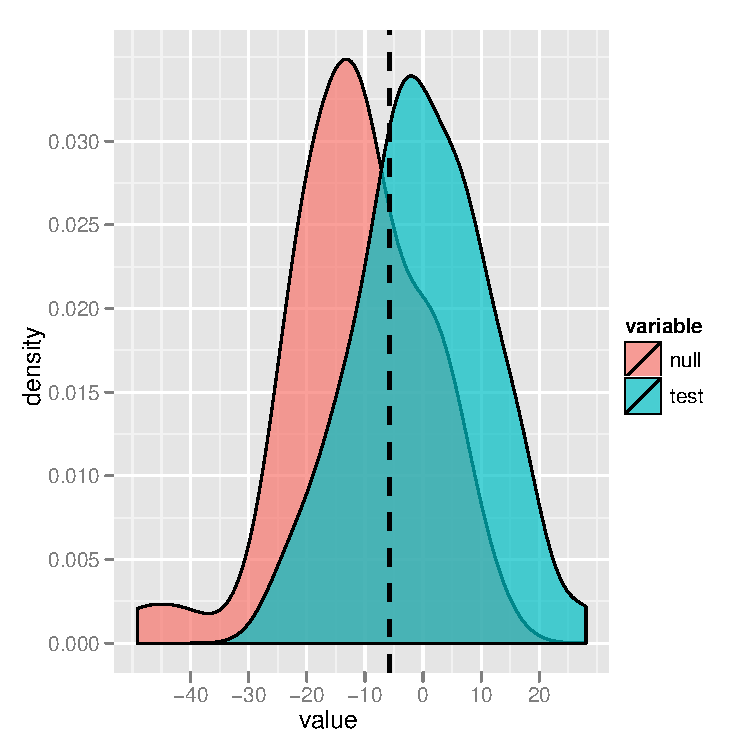
\includegraphics{earlyburst_fig} 

\end{kframe}}
\end{knitrout}

\caption{Early burst models can be very almost impossible to distinguish from OU models when each has been parameterized from the same data.}\label{fig:eb}
\end{figure}

\section{Utilities}
To implement the pmc package over a variety of methods, I have written an abstraction layer for phylogenetic comparative methods. A few of those methods may be useful to others, so I have made them accessible from the package and introduce them here.  Using the simulated tree and data from the early burst example above, we can swap between formats of both the tree and the data at whim, something that might be useful for anyone using both ouch and the other methods.  
\begin{knitrout}
\definecolor{shadecolor}{rgb}{.97, .97, .97}{\color{fgcolor}\begin{kframe}
\begin{flushleft}
\ttfamily\noindent
\hlsymbol{ouch}{\ }\hlassignement{\usebox{\hlnormalsizeboxlessthan}-}{\ }\hlfunctioncall{format\usebox{\hlnormalsizeboxunderscore}data}\hlkeyword{(}\hlsymbol{simtree}\hlkeyword{,}{\ }\hlsymbol{dat}\hlkeyword{)}\hspace*{\fill}\\
\hlstd{}\hlsymbol{ape}{\ }\hlassignement{\usebox{\hlnormalsizeboxlessthan}-}{\ }\hlfunctioncall{format\usebox{\hlnormalsizeboxunderscore}data}\hlkeyword{(}\hlsymbol{ouch}\hlkeyword{\usebox{\hlnormalsizeboxdollar}}\hlsymbol{tree}\hlkeyword{,}{\ }\hlsymbol{ouch}\hlkeyword{\usebox{\hlnormalsizeboxdollar}}\hlsymbol{dat}\hlkeyword{)}\mbox{}
\normalfont
\end{flushleft}
\end{kframe}}
\end{knitrout}


This format swapping is handled automatically in pmc's generic function for fitting phylogenetic models.  This function acts as a wrapper around existing methods, allowing the user to call the ouch methods while passing in data in either ouch or geiger format.   
\begin{knitrout}
\definecolor{shadecolor}{rgb}{.97, .97, .97}{\color{fgcolor}\begin{kframe}
\begin{flushleft}
\ttfamily\noindent
\hlsymbol{A}{\ }\hlassignement{\usebox{\hlnormalsizeboxlessthan}-}{\ }\hlfunctioncall{pmc\usebox{\hlnormalsizeboxunderscore}fit}\hlkeyword{(}\hlsymbol{ape}\hlkeyword{\usebox{\hlnormalsizeboxdollar}}\hlsymbol{tree}\hlkeyword{,}{\ }\hlsymbol{ape}\hlkeyword{\usebox{\hlnormalsizeboxdollar}}\hlsymbol{data}\hlkeyword{,}{\ }\hlargument{model}{\ }\hlargument{=}{\ }\hlstring{"{}BM"{}}\hlkeyword{)}\mbox{}
\normalfont
\end{flushleft}
\begin{verbatim}
## Fitting  BM model:
\end{verbatim}
\begin{flushleft}
\ttfamily\noindent
\hlsymbol{B}{\ }\hlassignement{\usebox{\hlnormalsizeboxlessthan}-}{\ }\hlfunctioncall{pmc\usebox{\hlnormalsizeboxunderscore}fit}\hlkeyword{(}\hlsymbol{simtree}\hlkeyword{,}{\ }\hlsymbol{dat}\hlkeyword{,}{\ }\hlargument{model}{\ }\hlargument{=}{\ }\hlstring{"{}hansen"{}}\hlkeyword{,}{\ }\hlargument{options}{\ }\hlargument{=}{\ }\hlfunctioncall{list}\hlkeyword{(}\hlargument{sqrt.alpha}{\ }\hlargument{=}{\ }\hlnumber{1}\hlkeyword{,}\hspace*{\fill}\\
\hlstd{}{\ }{\ }{\ }{\ }\hlargument{sigma}{\ }\hlargument{=}{\ }\hlnumber{1}\hlkeyword{,}{\ }\hlargument{regimes}{\ }\hlargument{=}{\ }\hlsymbol{regimes}\hlkeyword{)}\hlkeyword{)}\mbox{}
\normalfont
\end{flushleft}
\end{kframe}}
\end{knitrout}

This function also returns an object of a class that matches the fitting method used.  This means that we can use commands such as:
\begin{knitrout}
\definecolor{shadecolor}{rgb}{.97, .97, .97}{\color{fgcolor}\begin{kframe}
\begin{flushleft}
\ttfamily\noindent
\hlsymbol{sim}{\ }\hlassignement{\usebox{\hlnormalsizeboxlessthan}-}{\ }\hlfunctioncall{simulate}\hlkeyword{(}\hlsymbol{A}\hlkeyword{)}\mbox{}
\normalfont
\end{flushleft}
\begin{verbatim}
## Error: no applicable method for 'simulate' applied to an object of class "fitContinuous"
\end{verbatim}
\begin{flushleft}
\ttfamily\noindent
\hlsymbol{newA}{\ }\hlassignement{\usebox{\hlnormalsizeboxlessthan}-}{\ }\hlfunctioncall{update}\hlkeyword{(}\hlsymbol{A}\hlkeyword{,}{\ }\hlfunctioncall{simulate}\hlkeyword{(}\hlsymbol{A}\hlkeyword{)}\hlkeyword{)}\mbox{}
\normalfont
\end{flushleft}
\begin{verbatim}
## Error: no applicable method for 'simulate' applied to an object of class "fitContinuous"
\end{verbatim}
\end{kframe}}
\end{knitrout}

which automatically recognize the kind of model fit and use that method to perform the simulations and updates. This object-oriented design already exists in ouch, so this simply extends the practice to other methods.  The fitted object stores the traits and phylogeny used to make the fit, as well as the model and fitting options, which can also help the user avoid reproducibility errors of mismatching data, fit options and results.


\subsection{Power Curves}

A seperate function, \texttt{treepower}, creates the power curves in Figure 6 of Boettiger et al, Evolution. This code illustrates how such an analysis is run with the pmc package.   
\begin{knitrout}
\definecolor{shadecolor}{rgb}{.97, .97, .97}{\color{fgcolor}\begin{kframe}
\begin{flushleft}
\ttfamily\noindent
\hlfunctioncall{require}\hlkeyword{(}\hlsymbol{pmc}\hlkeyword{)}\hspace*{\fill}\\
\hlstd{}\hlfunctioncall{require}\hlkeyword{(}\hlsymbol{TreeSim}\hlkeyword{)}\hspace*{\fill}\\
\hlstd{}\hlfunctioncall{require}\hlkeyword{(}\hlsymbol{ouch}\hlkeyword{)}\hspace*{\fill}\\
\hlstd{}\hlsymbol{nboot}{\ }\hlassignement{\usebox{\hlnormalsizeboxlessthan}-}{\ }\hlnumber{200}\hspace*{\fill}\\
\hlstd{}\hlsymbol{cpu}{\ }\hlassignement{\usebox{\hlnormalsizeboxlessthan}-}{\ }\hlnumber{4}\hspace*{\fill}\\
\hlstd{}\hlsymbol{alpha}{\ }\hlassignement{\usebox{\hlnormalsizeboxlessthan}-}{\ }\hlfunctioncall{c}\hlkeyword{(}\hlnumber{0.01}\hlkeyword{,}{\ }\hlnumber{0.1}\hlkeyword{,}{\ }\hlnumber{1}\hlkeyword{,}{\ }\hlnumber{1.5}\hlkeyword{,}{\ }\hlnumber{2}\hlkeyword{,}{\ }\hlnumber{5}\hlkeyword{,}{\ }\hlnumber{10}\hlkeyword{,}{\ }\hlnumber{20}\hlkeyword{)}\hspace*{\fill}\\
\hlstd{}\hlsymbol{n}{\ }\hlassignement{\usebox{\hlnormalsizeboxlessthan}-}{\ }\hlfunctioncall{c}\hlkeyword{(}\hlnumber{5}\hlkeyword{,}{\ }\hlnumber{10}\hlkeyword{,}{\ }\hlnumber{20}\hlkeyword{,}{\ }\hlnumber{50}\hlkeyword{,}{\ }\hlnumber{100}\hlkeyword{)}\hspace*{\fill}\\
\hlstd{}\hlsymbol{lambda}{\ }\hlassignement{\usebox{\hlnormalsizeboxlessthan}-}{\ }\hlfunctioncall{c}\hlkeyword{(}\hlnumber{0.25}\hlkeyword{,}{\ }\hlnumber{0.5}\hlkeyword{,}{\ }\hlnumber{0.75}\hlkeyword{,}{\ }\hlnumber{1}\hlkeyword{)}\hspace*{\fill}\\
\hlstd{}\hlcomment{\usebox{\hlnormalsizeboxhash}{\ }size{\ }simulations}\hspace*{\fill}\\
\hlstd{}\hlsymbol{size}{\ }\hlassignement{\usebox{\hlnormalsizeboxlessthan}-}{\ }\hlfunctioncall{lapply}\hlkeyword{(}\hlnumber{1}\hlkeyword{:}\hlfunctioncall{length}\hlkeyword{(}\hlsymbol{n}\hlkeyword{)}\hlkeyword{,}{\ }\hlkeyword{function}\hlkeyword{(}\hlformalargs{i}\hlkeyword{)}{\ }\hlkeyword{\usebox{\hlnormalsizeboxopenbrace}}\hspace*{\fill}\\
\hlstd{}{\ }{\ }{\ }{\ }\hlsymbol{simtree}{\ }\hlassignement{\usebox{\hlnormalsizeboxlessthan}-}{\ }\hlfunctioncall{sim.bd.taxa}\hlkeyword{(}\hlargument{n}{\ }\hlargument{=}{\ }\hlsymbol{n}\hlkeyword{[}\hlsymbol{i}\hlkeyword{]}\hlkeyword{,}{\ }\hlargument{numbsim}{\ }\hlargument{=}{\ }\hlnumber{1}\hlkeyword{,}{\ }\hlargument{lambda}{\ }\hlargument{=}{\ }\hlnumber{1}\hlkeyword{,}\hspace*{\fill}\\
\hlstd{}{\ }{\ }{\ }{\ }{\ }{\ }{\ }{\ }\hlargument{mu}{\ }\hlargument{=}{\ }\hlnumber{0}\hlkeyword{,}{\ }\hlargument{frac}{\ }\hlargument{=}{\ }\hlnumber{1}\hlkeyword{,}{\ }\hlargument{complete}{\ }\hlargument{=}{\ }\hlnumber{FALSE}\hlkeyword{,}{\ }\hlargument{stochsampling}{\ }\hlargument{=}{\ }\hlnumber{FALSE}\hlkeyword{)}\hlkeyword{[[}\hlnumber{1}\hlkeyword{]}\hlkeyword{]}\hlkeyword{[[}\hlnumber{1}\hlkeyword{]}\hlkeyword{]}\hspace*{\fill}\\
\hlstd{}{\ }{\ }{\ }{\ }\hlfunctioncall{treepower}\hlkeyword{(}\hlfunctioncall{ape2ouch}\hlkeyword{(}\hlsymbol{simtree}\hlkeyword{)}\hlkeyword{,}{\ }\hlargument{nboot}{\ }\hlargument{=}{\ }\hlsymbol{nboot}\hlkeyword{,}{\ }\hlargument{cpu}{\ }\hlargument{=}{\ }\hlsymbol{cpu}\hlkeyword{,}\hspace*{\fill}\\
\hlstd{}{\ }{\ }{\ }{\ }{\ }{\ }{\ }{\ }\hlargument{alpha}{\ }\hlargument{=}{\ }\hlsymbol{alpha}\hlkeyword{)}\hspace*{\fill}\\
\hlstd{}\hlkeyword{\usebox{\hlnormalsizeboxclosebrace}}\hlkeyword{)}\mbox{}
\normalfont
\end{flushleft}
\begin{verbatim}
## Library pmc loaded.
\end{verbatim}
\begin{verbatim}
## Library pmc loaded.
\end{verbatim}
\begin{verbatim}
## Library pmc loaded.
\end{verbatim}
\begin{verbatim}
## Library pmc loaded.
\end{verbatim}
\begin{verbatim}
## Library pmc loaded.
\end{verbatim}
\begin{flushleft}
\ttfamily\noindent
\hlcomment{\usebox{\hlnormalsizeboxhash}\usebox{\hlnormalsizeboxhash}{\ }Shape{\ }simulations}\hspace*{\fill}\\
\hlstd{}\hlsymbol{N}{\ }\hlassignement{\usebox{\hlnormalsizeboxlessthan}-}{\ }\hlnumber{50}{\ }{\ }\hlcomment{\usebox{\hlnormalsizeboxhash}\usebox{\hlnormalsizeboxhash}{\ }number{\ }of{\ }taxa{\ }fixed{\ }to{\ }50}\hspace*{\fill}\\
\hlstd{}\hlsymbol{shape}{\ }\hlassignement{\usebox{\hlnormalsizeboxlessthan}-}{\ }\hlfunctioncall{lapply}\hlkeyword{(}\hlnumber{1}\hlkeyword{:}\hlfunctioncall{length}\hlkeyword{(}\hlsymbol{lambda}\hlkeyword{)}\hlkeyword{,}{\ }\hlkeyword{function}\hlkeyword{(}\hlformalargs{i}\hlkeyword{)}{\ }\hlkeyword{\usebox{\hlnormalsizeboxopenbrace}}\hspace*{\fill}\\
\hlstd{}{\ }{\ }{\ }{\ }\hlsymbol{simtree}{\ }\hlassignement{\usebox{\hlnormalsizeboxlessthan}-}{\ }\hlfunctioncall{sim.bd.taxa}\hlkeyword{(}\hlargument{n}{\ }\hlargument{=}{\ }\hlsymbol{N}\hlkeyword{,}{\ }\hlargument{numbsim}{\ }\hlargument{=}{\ }\hlnumber{1}\hlkeyword{,}{\ }\hlargument{lambda}{\ }\hlargument{=}{\ }\hlnumber{1}\hlkeyword{,}\hspace*{\fill}\\
\hlstd{}{\ }{\ }{\ }{\ }{\ }{\ }{\ }{\ }\hlargument{mu}{\ }\hlargument{=}{\ }\hlnumber{0}\hlkeyword{,}{\ }\hlargument{frac}{\ }\hlargument{=}{\ }\hlnumber{1}\hlkeyword{,}{\ }\hlargument{complete}{\ }\hlargument{=}{\ }\hlnumber{FALSE}\hlkeyword{,}{\ }\hlargument{stochsampling}{\ }\hlargument{=}{\ }\hlnumber{FALSE}\hlkeyword{)}\hlkeyword{[[}\hlnumber{1}\hlkeyword{]}\hlkeyword{]}\hlkeyword{[[}\hlnumber{1}\hlkeyword{]}\hlkeyword{]}\hspace*{\fill}\\
\hlstd{}{\ }{\ }{\ }{\ }\hlsymbol{simtree}{\ }\hlassignement{\usebox{\hlnormalsizeboxlessthan}-}{\ }\hlfunctioncall{lambdaTree}\hlkeyword{(}\hlsymbol{simtree}\hlkeyword{,}{\ }\hlsymbol{lambda}\hlkeyword{[}\hlsymbol{i}\hlkeyword{]}\hlkeyword{)}\hspace*{\fill}\\
\hlstd{}{\ }{\ }{\ }{\ }\hlfunctioncall{treepower}\hlkeyword{(}\hlfunctioncall{ape2ouch}\hlkeyword{(}\hlsymbol{simtree}\hlkeyword{)}\hlkeyword{,}{\ }\hlargument{nboot}{\ }\hlargument{=}{\ }\hlsymbol{nboot}\hlkeyword{,}{\ }\hlargument{cpu}{\ }\hlargument{=}{\ }\hlsymbol{cpu}\hlkeyword{,}\hspace*{\fill}\\
\hlstd{}{\ }{\ }{\ }{\ }{\ }{\ }{\ }{\ }\hlargument{alpha}{\ }\hlargument{=}{\ }\hlsymbol{alpha}\hlkeyword{)}\hspace*{\fill}\\
\hlstd{}\hlkeyword{\usebox{\hlnormalsizeboxclosebrace}}\hlkeyword{)}\mbox{}
\normalfont
\end{flushleft}
\begin{verbatim}
## Library pmc loaded.
\end{verbatim}
\begin{verbatim}
## Library pmc loaded.
\end{verbatim}
\begin{verbatim}
## Library pmc loaded.
\end{verbatim}
\begin{verbatim}
## Library pmc loaded.
\end{verbatim}
\end{kframe}}
\end{knitrout}




\begin{figure}
\begin{center}
\begin{knitrout}
\definecolor{shadecolor}{rgb}{.97, .97, .97}{\color{fgcolor}\begin{kframe}
\begin{flushleft}
\ttfamily\noindent
\hlsymbol{plot\usebox{\hlnormalsizeboxunderscore}size}{\ }\hlassignement{\usebox{\hlnormalsizeboxlessthan}-}{\ }\hlkeyword{function}\hlkeyword{(}\hlkeyword{)}{\ }\hlkeyword{\usebox{\hlnormalsizeboxopenbrace}}\hspace*{\fill}\\
\hlstd{}{\ }{\ }{\ }{\ }\hlsymbol{k}{\ }\hlassignement{\usebox{\hlnormalsizeboxlessthan}-}{\ }\hlfunctioncall{length}\hlkeyword{(}\hlsymbol{n}\hlkeyword{)}\hspace*{\fill}\\
\hlstd{}{\ }{\ }{\ }{\ }\hlfunctioncall{plot}\hlkeyword{(}\hlnumber{1}\hlkeyword{,}{\ }\hlnumber{1}\hlkeyword{,}{\ }\hlargument{type}{\ }\hlargument{=}{\ }\hlstring{"{}n"{}}\hlkeyword{,}{\ }\hlargument{xlim}{\ }\hlargument{=}{\ }\hlfunctioncall{c}\hlkeyword{(}\hlfunctioncall{min}\hlkeyword{(}\hlsymbol{alpha}\hlkeyword{)}\hlkeyword{,}{\ }\hlfunctioncall{max}\hlkeyword{(}\hlsymbol{alpha}\hlkeyword{)}\hlkeyword{)}\hlkeyword{,}\hspace*{\fill}\\
\hlstd{}{\ }{\ }{\ }{\ }{\ }{\ }{\ }{\ }\hlargument{ylim}{\ }\hlargument{=}{\ }\hlfunctioncall{c}\hlkeyword{(}\hlnumber{0}\hlkeyword{,}{\ }\hlnumber{1}\hlkeyword{)}\hlkeyword{,}{\ }\hlargument{main}{\ }\hlargument{=}{\ }\hlstring{"{}Power{\ }by{\ }tree{\ }size"{}}\hlkeyword{,}{\ }\hlargument{log}{\ }\hlargument{=}{\ }\hlstring{"{}x"{}}\hlkeyword{,}\hspace*{\fill}\\
\hlstd{}{\ }{\ }{\ }{\ }{\ }{\ }{\ }{\ }\hlargument{xlab}{\ }\hlargument{=}{\ }\hlstring{"{}alpha"{}}\hlkeyword{,}{\ }\hlargument{ylab}{\ }\hlargument{=}{\ }\hlstring{"{}power"{}}\hlkeyword{)}\hspace*{\fill}\\
\hlstd{}{\ }{\ }{\ }{\ }\hlkeyword{for}{\ }\hlkeyword{(}\hlsymbol{i}{\ }\hlkeyword{in}{\ }\hlnumber{1}\hlkeyword{:}\hlsymbol{k}\hlkeyword{)}{\ }\hlkeyword{\usebox{\hlnormalsizeboxopenbrace}}\hspace*{\fill}\\
\hlstd{}{\ }{\ }{\ }{\ }{\ }{\ }{\ }{\ }\hlcomment{\usebox{\hlnormalsizeboxhash}\usebox{\hlnormalsizeboxhash}{\ }skip{\ }the{\ }last{\ }2,{\ }which{\ }haven\usebox{\hlnormalsizeboxsinglequote}t{\ }converged}\hspace*{\fill}\\
\hlstd{}{\ }{\ }{\ }{\ }{\ }{\ }{\ }{\ }\hlfunctioncall{points}\hlkeyword{(}\hlsymbol{alpha}\hlkeyword{,}{\ }\hlsymbol{size}\hlkeyword{[[}\hlsymbol{i}\hlkeyword{]}\hlkeyword{]}\hlkeyword{\usebox{\hlnormalsizeboxdollar}}\hlsymbol{power}\hlkeyword{,}{\ }\hlargument{pch}{\ }\hlargument{=}{\ }\hlnumber{16}\hlkeyword{,}{\ }\hlargument{col}{\ }\hlargument{=}{\ }\hlsymbol{i}\hlkeyword{)}\hspace*{\fill}\\
\hlstd{}{\ }{\ }{\ }{\ }{\ }{\ }{\ }{\ }\hlfunctioncall{lines}\hlkeyword{(}\hlsymbol{alpha}\hlkeyword{,}{\ }\hlsymbol{size}\hlkeyword{[[}\hlsymbol{i}\hlkeyword{]}\hlkeyword{]}\hlkeyword{\usebox{\hlnormalsizeboxdollar}}\hlsymbol{power}\hlkeyword{,}{\ }\hlargument{col}{\ }\hlargument{=}{\ }\hlsymbol{i}\hlkeyword{)}\hspace*{\fill}\\
\hlstd{}{\ }{\ }{\ }{\ }\hlkeyword{\usebox{\hlnormalsizeboxclosebrace}}\hspace*{\fill}\\
\hlstd{}{\ }{\ }{\ }{\ }\hlfunctioncall{legend}\hlkeyword{(}\hlstring{"{}topleft"{}}\hlkeyword{,}{\ }\hlfunctioncall{paste}\hlkeyword{(}\hlsymbol{n}\hlkeyword{,}{\ }\hlstring{"{}taxa"{}}\hlkeyword{)}\hlkeyword{,}{\ }\hlargument{col}{\ }\hlargument{=}{\ }\hlnumber{1}\hlkeyword{:}\hlsymbol{k}\hlkeyword{,}{\ }\hlargument{pch}{\ }\hlargument{=}{\ }\hlnumber{16}\hlkeyword{)}\hspace*{\fill}\\
\hlstd{}\hspace*{\fill}\\
\hlstd{}\hlkeyword{\usebox{\hlnormalsizeboxclosebrace}}\hspace*{\fill}\\
\hlstd{}\hlfunctioncall{plot\usebox{\hlnormalsizeboxunderscore}size}\hlkeyword{(}\hlkeyword{)}\mbox{}
\normalfont
\end{flushleft}


\centering{}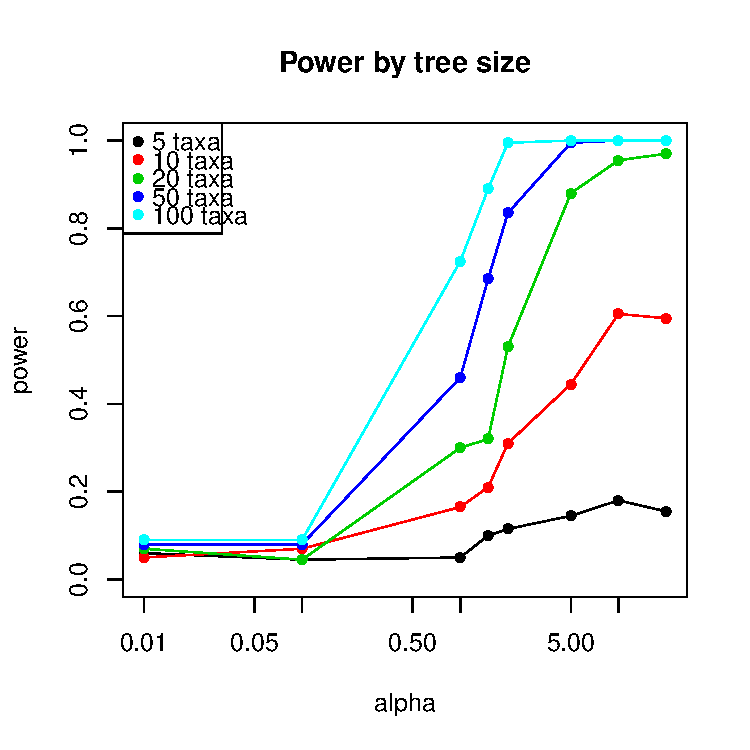
\includegraphics{Fig6a} 

\end{kframe}}
\end{knitrout}

\end{center}
\caption{}
\label{fig:sixa}
\end{figure}



\begin{figure}
\begin{center}
\begin{knitrout}
\definecolor{shadecolor}{rgb}{.97, .97, .97}{\color{fgcolor}\begin{kframe}
\begin{flushleft}
\ttfamily\noindent
\hspace*{\fill}\\
\hlstd{}\hspace*{\fill}\\
\hlstd{}\hlsymbol{plot\usebox{\hlnormalsizeboxunderscore}shape}{\ }\hlassignement{\usebox{\hlnormalsizeboxlessthan}-}{\ }\hlkeyword{function}\hlkeyword{(}\hlkeyword{)}{\ }\hlkeyword{\usebox{\hlnormalsizeboxopenbrace}}\hspace*{\fill}\\
\hlstd{}{\ }{\ }{\ }{\ }\hlfunctioncall{plot}\hlkeyword{(}\hlnumber{1}\hlkeyword{,}{\ }\hlnumber{1}\hlkeyword{,}{\ }\hlargument{type}{\ }\hlargument{=}{\ }\hlstring{"{}n"{}}\hlkeyword{,}{\ }\hlargument{xlim}{\ }\hlargument{=}{\ }\hlfunctioncall{c}\hlkeyword{(}\hlfunctioncall{min}\hlkeyword{(}\hlsymbol{alpha}\hlkeyword{)}\hlkeyword{,}{\ }\hlfunctioncall{max}\hlkeyword{(}\hlsymbol{alpha}\hlkeyword{)}\hlkeyword{)}\hlkeyword{,}\hspace*{\fill}\\
\hlstd{}{\ }{\ }{\ }{\ }{\ }{\ }{\ }{\ }\hlargument{ylim}{\ }\hlargument{=}{\ }\hlfunctioncall{c}\hlkeyword{(}\hlnumber{0}\hlkeyword{,}{\ }\hlnumber{1}\hlkeyword{)}\hlkeyword{,}{\ }\hlargument{main}{\ }\hlargument{=}{\ }\hlstring{"{}Power{\ }by{\ }tree{\ }topology"{}}\hlkeyword{,}\hspace*{\fill}\\
\hlstd{}{\ }{\ }{\ }{\ }{\ }{\ }{\ }{\ }\hlargument{log}{\ }\hlargument{=}{\ }\hlstring{"{}x"{}}\hlkeyword{,}{\ }\hlargument{xlab}{\ }\hlargument{=}{\ }\hlstring{"{}alpha"{}}\hlkeyword{,}{\ }\hlargument{ylab}{\ }\hlargument{=}{\ }\hlstring{"{}power"{}}\hlkeyword{)}\hspace*{\fill}\\
\hlstd{}{\ }{\ }{\ }{\ }\hlsymbol{k}{\ }\hlassignement{\usebox{\hlnormalsizeboxlessthan}-}{\ }\hlfunctioncall{length}\hlkeyword{(}\hlsymbol{lambda}\hlkeyword{)}\hspace*{\fill}\\
\hlstd{}{\ }{\ }{\ }{\ }\hlkeyword{for}{\ }\hlkeyword{(}\hlsymbol{i}{\ }\hlkeyword{in}{\ }\hlnumber{1}\hlkeyword{:}\hlsymbol{k}\hlkeyword{)}{\ }\hlkeyword{\usebox{\hlnormalsizeboxopenbrace}}\hspace*{\fill}\\
\hlstd{}{\ }{\ }{\ }{\ }{\ }{\ }{\ }{\ }\hlfunctioncall{points}\hlkeyword{(}\hlsymbol{alpha}\hlkeyword{,}{\ }\hlsymbol{shape}\hlkeyword{[[}\hlsymbol{i}\hlkeyword{]}\hlkeyword{]}\hlkeyword{\usebox{\hlnormalsizeboxdollar}}\hlsymbol{power}\hlkeyword{,}{\ }\hlargument{pch}{\ }\hlargument{=}{\ }\hlnumber{16}\hlkeyword{,}{\ }\hlargument{col}{\ }\hlargument{=}{\ }\hlsymbol{i}\hlkeyword{)}\hspace*{\fill}\\
\hlstd{}{\ }{\ }{\ }{\ }{\ }{\ }{\ }{\ }\hlfunctioncall{lines}\hlkeyword{(}\hlsymbol{alpha}\hlkeyword{,}{\ }\hlsymbol{shape}\hlkeyword{[[}\hlsymbol{i}\hlkeyword{]}\hlkeyword{]}\hlkeyword{\usebox{\hlnormalsizeboxdollar}}\hlsymbol{power}\hlkeyword{,}{\ }\hlargument{col}{\ }\hlargument{=}{\ }\hlsymbol{i}\hlkeyword{)}\hspace*{\fill}\\
\hlstd{}{\ }{\ }{\ }{\ }\hlkeyword{\usebox{\hlnormalsizeboxclosebrace}}\hspace*{\fill}\\
\hlstd{}{\ }{\ }{\ }{\ }\hlfunctioncall{legend}\hlkeyword{(}\hlstring{"{}topleft"{}}\hlkeyword{,}{\ }\hlfunctioncall{paste}\hlkeyword{(}\hlsymbol{lambda}\hlkeyword{,}{\ }\hlstring{"{}lambda"{}}\hlkeyword{)}\hlkeyword{,}{\ }\hlargument{col}{\ }\hlargument{=}{\ }\hlnumber{1}\hlkeyword{:}\hlsymbol{k}\hlkeyword{,}\hspace*{\fill}\\
\hlstd{}{\ }{\ }{\ }{\ }{\ }{\ }{\ }{\ }\hlargument{pch}{\ }\hlargument{=}{\ }\hlnumber{16}\hlkeyword{)}\hspace*{\fill}\\
\hlstd{}\hlkeyword{\usebox{\hlnormalsizeboxclosebrace}}\hspace*{\fill}\\
\hlstd{}\hlfunctioncall{plot\usebox{\hlnormalsizeboxunderscore}shape}\hlkeyword{(}\hlkeyword{)}\mbox{}
\normalfont
\end{flushleft}


\centering{}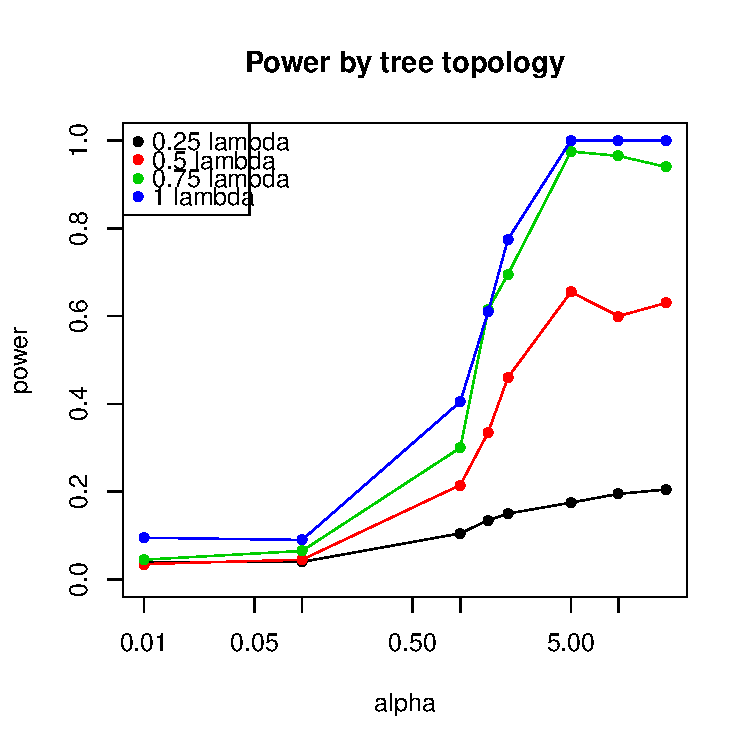
\includegraphics{Fig6b} 

\end{kframe}}
\end{knitrout}

\end{center}
\label{fig:sixb}
\end{figure}



\section*{ }%bibliography
\bibliographystyle{elsarticle-harv}
%\bibliography{/home/cboettig/Documents/Mendeley/bib/library}
\bibliography{pmc_tutorial}

\end{document}

